\documentclass[12pt,a4paper]{article}
\usepackage[utf8]{inputenc}
\usepackage[english, ngerman]{babel}
\usepackage{amsmath}
\usepackage{amsfonts}
\usepackage{amssymb}
\usepackage{graphicx}
\usepackage[section]{placeins}
\usepackage{url}
%\usepackage{times}
\usepackage{hyperref}
\usepackage{tabularx}
\usepackage{flafter}

%\usepackage{apager}
\usepackage[style=authoryear,bibstyle=apa,backend=biber]{biblatex}
\DeclareLanguageMapping{ngerman}{ngerman-apa}
\DefineBibliographyStrings{ngerman}{andothers = {{et\,al\adddot}},}
\DefineBibliographyStrings{ngerman}{and = {{\&}},}
\DefineBibliographyStrings{ngerman}{references = {Literaturverzeichnis}
}%umbennen Litertaur zu Literaturverzeichnis
\setcounter{smartand}{0}
\bibliography{lit_master}

\usepackage[font=small]{caption}
\captionsetup[figure]{labelfont=it, labelsep=period}
\captionsetup[table]{textfont=it,singlelinecheck=false,labelsep=newline,format=plain,justification=justified}
\usepackage[a4paper,top=3cm,bottom=3cm,left=3cm,right=4cm]{geometry}
\usepackage{setspace}
\onehalfspacing

\author{Iryna Karpyuk \\
Matrikelnummer: 4222981}
\title{Die Einschätzung der Erziehungs- und Bildungspartnerschaft zwischen pädagogischen Fachkräften und Familien durch die Eltern am Beispiel der FRÖBEL-Kindertageseinrichtungen}
\begin{document}
\begin{titlepage}

\normalsize

\begin{center}
Freie Universität Berlin \\
Fachbereich Erziehungswissenschaft und Psychologie\\
Masterarbeit im Masterstudiengang Bildungswissenschaft
\end{center}

\vspace{30pt}

\begin{center}
%\fontfamily{phv}\selectfont{
\LARGE%}
\\  
\vspace{50pt}
 \end{center}
                         
\normalsize  
\begin{center}
Erstgutachterin:  Prof. Dr. Yvonne Anders\\
Zweitgutachterin:  Dr. Axinja Hachfeld\\
\vspace{10pt}
Vorgelegt von\\ 
Iryna Karpyuk \\
Matrikelnummer: 4222981\\
\end{center}                  
Wörter im Textteil: [Anzahl Wörter]\\     

\begin{center}
\normalsize
\vspace{150pt}

Berlin, 9.Feb.2015
\end{center}
\end{titlepage}
\normalsize                                              
\pagebreak

%\maketitle

\begin{abstract}
This thesis deals with the partnership in upbringing and education between
pedagogues and parents in the FRÖBEL kindergarden institutions. This study
investigates the question which homogenous dimensions emerge from the sub scale
``collaboration with parents'' and how the cooperation between the pedagogues
and the families is evaluated by the parents.
The basis of this work are 2579 questionaires given to parents in which the
families could asses the cooperation.
The results illustrate that the majority of the parents expressed satisfaction
with the collaboration between the pedagogues and the families in the FRÖBEL
kindergarten institutions. Additionally one dimension ``collaboration with
parents'' was extracted in the data structure by exploritatory factor analysis.
%Die vorliegende Arbeit beschäftigt sich mit der Erziehungs- und Bildungspartnerschaft zwischen den pädagogischen Fachkräften und Eltern in den FRÖBEL-Kindertageseinrichtungen. Die Studie geht der Frage nach, welche homogenen Dimensionen sich in der Subskala „Zusammenarbeit mit Familien“ herausbilden lassen und wie die Kooperation zwischen den pädagogischen Fachkräften und den Familien aus der Sicht der Eltern beurteilt wird.
%Die Datengrundlage bilden 2579 Elternfragebögen, anhand deren Eltern die Möglichkeit bekommen haben, die Zusammenarbeit einzuschätzen.
%Die Befunde veranschaulichen, dass sich die Mehrheit der Eltern positiv bezüglich der Zusammenarbeit zwischen pädagogischen Fachkräften und Familien in den FRÖBEL-Einrichtungen äußerten. Weiterhin ließ sich in der Datenstruktur mittels der exploratorischen Faktorenanalyse eine Dimension „Zusammenarbeit mit Familien“ herausbilden.
\end{abstract}

\pagebreak

\tableofcontents
\pagebreak
\listoffigures
\pagebreak
\listoftables
\pagebreak

\begin{titlepage}
\end{titlepage}
\vspace*{\fill}
\begin{Huge}\noindent
I: Einleitung und theoretischer Rahmen der Arbeit
\end{Huge}
\vspace*{\fill}
\pagebreak

\section{Einleitung}
\textit{"`Es macht keinen Sinn, ein Kind zu erziehen, ohne dabei die für das Kind bedeutendsten Menschen zu berücksichtigen"'}
 (Tina Bruce, 1977).\\
 
 
\noindent Heutzutage wachsen Kinder vorwiegend in den zwei Systemen "`Familie"' und "`Kindertageseinrichtung"' auf. Die Aufgabe der beiden Systeme besteht nicht nur darin, die Kinder zu erziehen, sondern in erster Linie sie in ihrer Entwicklung bestmöglich zu fördern und zu unterstützen. Um dies zu erreichen, sollten die beiden Systeme bewusst eine wechselseitige Kooperation anstreben und sich gegenseitig in der Erziehung, Bildung und Betreuung der Kinder ergänzen.
	  
Die Zusammenarbeit\footnote{In der vorliegenden Arbeit werden die Begriffe "`Zusammenarbeit mit Familien"' und "`Erziehungs- und Bildungspartnerschaft"' als Synonyme verwendet.} zwischen Familien und pä\-da\-go\-gisch\-en Fach\-kräf\-ten stellt eine der primären Aufgaben der Kindertageseinrichtungen dar. Sie bildet neben den zwei wichtigsten Aufgabenspektren der Erzieher/-innen: der "`direkten"' pä\-da\-go\-gisch\-en Arbeit am Kind und der Notwendigkeit der systematischen, institutionellen Vernetzung mit anderen Einrichtungen, einen dritten wesentlichen Aspekt moderner Kindergartenpädagogik (Kasüschke \& Fröhlich-Gildhoff, 2008, S. 141). Dass die Zusammenarbeit mit den Eltern in den Kindergärten einen so hohen Stellenwert einnimmt, ist nicht zuletzt der gestiegenen Bedeutung der vorschulischen Bildung, Betreuung und Erziehung zu verdanken. Als Folge wird in der heutigen Gesellschaft ein immer größerer Wert auf eine gute Zusammenarbeit zwischen den Kindertagesstätten und den Eltern gelegt. In diesem Zusammenhang hat die Elternarbeit in den letzten Jahren eine grundlegende Wandlung erfahren. Für lange Zeit wurde die Zusammenarbeit mit Familien für eine als unnötig betrachtete Zusatzbelastung für die pädagogischen Fachkräfte gehalten. Erst seit den 80er Jahren rückt sie immer mehr in den Fokus der Öffentlichkeit. Diesen geschichtlichen Wandel grob zu skizzieren, ist ein Teil der Arbeit. Das Ziel der Auseinandersetzung mit den geschichtlich und gesellschaftlich stattgefundenen Veränderungen (Kapitel 2) ist zum einen, die fortdauernde Notwendigkeit von Veränderung und Anpassung in der Elternarbeit zu betonen, aber auch die zunehmende Signifikanz des Themas damit zu untermauern.

Die zweite Aufgabe dieser Arbeit bestand darin, einen Einblick in die bisherigen, empirisch gestützten Erkenntnisse zu diesem Thema zu ermöglichen. Die Recherche zum aktuellen Forschungsstand hat ergeben, dass sich sowohl in der nationalen als auch in der internationalen Forschung wenig mit der Zusammenarbeit mit Familien in den Kindertageseinrichtungen aus der Sicht der Eltern beschäftigt wurde. Dies betrifft insbesondere den deutschsprachigen Raum.  Es finden sich insgesamt nur wenige empirische Studien in diesem Bereich. Die meisten davon sind zudem entweder wenig aktuell oder enthalten zu kleine Stichproben bzw. sind thematisch sehr eng angelegt. Auch im angloamerikanischen Sprachraum beschäftigen sich die meisten Untersuchungen kaum mit der Zusammenarbeit mit Familien im regulären Kindergartenalltag. Sie sind eher auf die Evaluation von Elternkursprogrammen in Kindergärten, auf die Zusammenarbeit in der Schule oder in der Kinderpsychotherapie ausgerichtet.  
Eine fundierte wissenschaftliche Auseinandersetzung mit der Thematik fehlt also nach wie vor trotz der wachsenden Bedeutsamkeit des ausgewählten Themas.

Aus diesem Grund liegt der Interessenschwerpunkt der vorliegenden Arbeit darin, den Lesern und Leserinnen die Relevanz und Notwendigkeit der Erziehungs- und Bildungspartnerschaft in den Kindertageseinrichtungen aufzuzeigen und damit zu einer intensiveren Auseinandersetzung mit dem Thema in der wissenschaftlichen Forschung anzuregen.
	
Der empirische Teil der Arbeit befasst sich mit einer explorativen Untersuchung zum Thema "`Zusammenarbeit mit Familien in Kindertageseinrichtungen"', die im Rahmen des Projekts "`FRÖBEL-Eltern- und Mitarbeiter/-innenbefragung 2013"' durchgeführt wurde. Das Interesse an den FRÖBEL-Kindergärten und deren Zusammenarbeit mit den Familien wurde während meines dreimonatigen Praktikums bei dem gemeinnützigen Verein FRÖBEL e.V\footnote{Der FRÖBEL e.V. ist ein anerkannter Träger der Jugendhilfe und betreibt Krippen, Kindergärten und Horte sowohl national (in mehreren Bundesländern Deutschlands) als auch international (Türkei, Australien). Aktuell werden ca. 12.000 Kinder in über 130 Einrichtungen betreut.} geweckt und im Laufe der Praktikumstätigkeiten, die vorwiegend im Bereich Qualitätsentwicklung in den Kindertageseinrichtungen lagen, in hohem Maße verstärkt.

In Anbetracht dessen, dass es speziell zu dem Thema "`Zusammenarbeit zwischen den Eltern und pädagogischen Fachkräften in FRÖBEL-Kin\-der\-ta\-ges\-ein\-rich\-tun\-gen"' bislang keine Forschungsergebnisse gibt, ist das zentrale Ziel dieser Arbeit, zu untersuchen, wie die Zusammenarbeit in den FRÖBEL-Kindergärten durch die Eltern bewertet wird. Im Vordergrund stehen die Fragen:
\begin{enumerate}
\item \textit{"`Wie schätzen die Eltern die Zusammenarbeit zwischen den pädagogischen Fachkräften und Familien in den FRÖBEL-Kindertageseinrichtungen ein?"'}
\item \textit{"`Welche homogenen Dimensionen (thematische Subkategorien) lassen sich in der Subskala "`Zusammenarbeit mit Familien"' des FRÖBEL-Eltern\-fra\-ge\-bo\-gens herausbilden?"'}
\end{enumerate}

Die vorliegende Arbeit ist in zwei große Blöcke eingeteilt. Im ersten, theoretischen Teil der Arbeit wird ein geschichtlicher Rückblick auf die Entwicklung von Erziehungs- und Bildungspartnerschaften mit Eltern gegeben. Im weiteren Schritt  wird aufgezeigt, dass der geschichtliche Wandel nicht nur auf die gesellschaftliche Wahrnehmung beschränkt ist, sondern sich auch in den rechtlichen Grundlagen und den Rahmenrichtlinien der Bundesländer zur Förderung der Bildungs- und Erziehungspartnerschaften widerspiegelt. Anschließend werden die wichtigsten, nach dem stattgefundenen Wandel neu definierten Inhalte der Erziehungs- und Bildungspartnerschaft benannt und einige gewichtige Argumente für die Relevanz der Zusammenarbeit mit den Familien vor dem Hintergrund dieser Veränderungen aufgeführt. Im Anschluss werden die bisherigen empirischen Forschungsergebnisse aus der gesichteten einschlägigen Literatur und weiteren analysierten Quellen wie fachliche Zeitschriften, Datenbanken etc. präsentiert.

Der zweite, empirische Teil der Arbeit zielt darauf, die bereits erwähnten Fragestellungen zu erforschen. Zunächst wird das Projekt "`FRÖBEL-Mitarbeiter/-innen- und Elternbefragung 2013"', das von den Mit\-arbei\-ter/-innen der FRÖBEL e.V. durchgeführt wurde, näher vorgestellt. Anschließend wird das methodische Vorgehen der empirischen Untersuchung erläutert. Das Kapitel umfasst zunächst Angaben zum Aufbau der Studie, zur Stichprobe und zur Erhebungsdurchführung. Darauf folgen Ausführungen zu den statistischen Analyseverfahren, wobei die explorative Faktorenanalyse als zentrales Verfahren verwendet wird. Im Weiteren werden die Ergebnisse dieser Studie zusammengefasst und die Befunde diskutiert. Abschließend werden einige Möglichkeiten für die weitere Forschung auf diesem Gebiet aufgezeigt.	
	

\section{Geschichtlicher Rückblick auf die Entwicklung von Erziehungs- und Bildungspartnerschaften mit Eltern}
In diesem Kapitel wird zunächst ein kurzer Einblick in die Anfänge der Zusammenarbeit mit Familien in Kindertageseinrichtungen gegeben. Ferner wird auf die Wandlung des Begriffes "`Elternarbeit"' -  von der Elternarbeit bis hin zur Erziehungs- und Bildungspartnerschaft - eingegangen.

	 Seit den 70er Jahren wird das Thema "`Zusammenarbeit mit den Eltern in  Kindertageseinrichtungen"' ver\-stärkt in der Fachdiskussion thematisiert und hat seitdem ständig an Bedeutung gewonnen. Das spiegelt sich in der pädagogischen Literatur deutlich wieder. Wenn man zurückblickt, stellt man fest, dass sich die Beziehung zwischen pädagogischen Fachkräften und Eltern im gesellschaftlichen Prozess mehrmals verändert hat. Bis Mitte des 19. Jahrhunderts verlief der Elterneinbezug in die pädagogische Arbeit nicht über die direkte Interaktion zwischen Pädagogen und Eltern, sondern anhand von literarischen Ratgebern zur Erziehung. In diesen Schriften ging es vor allem um die Belehrung und Unterweisung der Eltern, denen der Status der Unterweisungsbedürftigen zugeschrieben wurde. Offene partnerschaftliche Absprachen in Erziehungsfragen zwischen beiden Akteuren werden erst seit kurzer Zeit und noch nicht durchgängig praktiziert (Wiezorek, 2006, S. 43).
	 
	Der erste Kontakt zwischen Eltern oder, genauer gesagt, zwischen Müttern und Erzieher/-innen kam zustande, als der Kleinkindpädagoge Friedrich Fröbel (1780-1852) um 1840 den ersten Kindergarten\footnote{Der erste Kindergarten wurde von Fröbel (1782-1852) 1840 in Blankenburg gegründet. Fröbels Pädagogik entstand aus der geistigen Bewegung der Romantik und des Idealismus. Für Fröbel stellte sich die Welt als sinnvolles Ganzes dar, und die Aufgabe der Erziehung sei es, den Menschen zum Einklang und zur Harmonie mit der Welt zu führen. Bereits 1851 wurden die neu eingerichteten Fröbel-Kindergärten für über 10 Jahre verboten (Berger, 2000, S. 10-22).} gründete. Mit der Konzeption des fröbelschen Kindergartens wurde zum ersten Mal in der Geschichte der Pädagogik das Ziel verfolgt, die familiäre Erziehung durch vorschulische Einrichtungen bewusst zu ergänzen. Fröbel sah seinen Kindergarten als Volksbildungsanstalt für Kinder, Eltern und Erzieher/-innen. Er regte auch die Gründung von Elternvereinen an, die die Initiatoren und Träger der ersten Kindergärten wurden.
	
Insbesondere betonte Fröbel die Rolle der Mutter mit ihren Eigenschaften, die für die Entwicklung des Kindes sehr förderlich sind. Mutter und Kind wurden von Fröbel als Einheit gesehen (Herrmann, 2007, S. 19-20). Allerdings, was die Zusammenarbeit mit Familien im heutigen Sinne\footnote{Die Eltern als Expertinnen und Experten für ihr Kind anzuerkennen, der regelmäßige wechselseitiger Dialog über die Entwicklung und Bildungsinteresse der Kinder, wertschätzende und respektvolle Grundhaltung gegenüber der Unterschiedlichkeit der familiären Lebensbedingungen und Lebensentwürfe, gegenseitiges Vertrauen etc. (Kieschnick, Marx \& Steinfeldt, 2014, S. 25-28).} im fröbelschen Kindergarten  anbelangt, war sie im 19. Jahrhundert lediglich in rudimentären Formen vorzufinden. Die Zusammenarbeit zu der Zeit ist aus reiner Notwendigkeit entstanden, das Funktionieren der Kindergartenarbeit zu sichern. Sie bestand hauptsächlich darin,  dass die Mütter ihre Kinder pünktlich in den Kindergarten bringen und abholen mussten. Gespräche über die Kinder waren nur dann vorgesehen, wenn etwas vorgefallen war. In solchen Fällen wurden die Mütter angehalten, ihre Kinder besser zu erziehen. Die Kooperation der Erzieher/-innen mit den Müttern ließ sich weithin als autoritär-hierarchisch bezeichnen (Thiersch, 2006, S. 82-83).

	In den 50er und 60er Jahren wurden Eltern weiterhin lediglich als Laien betrachtet und im Kindergarten eher am Rande einbezogen. Die Kooperation mit ihnen beschränkte sich nur darauf, zu zeigen wie inkompetent und pädagogisch ungebildet sie sind. Bis in die 80er Jahre gaben die Institutionen die Bedingungen vor, denen sich Eltern in der Regel zu fügen hatten. Die Anpassung der Eltern an die Vorgaben der Einrichtung war selbstverständlich. Zum Beispiel in der DDR durften die Eltern oft keine Gruppenräume betreten und in Westdeutschland gab es bis weit in die 60er Jahre hinein weder Elternbeiräte noch andere Formen von Elternmitsprache (Klein \& Vogt, 2008, S. 22).
	
	Eine Wende in der Zusammenarbeit zwischen Kindertageseinrichtungen und Eltern lässt sich seit 1986 in Westdeutschland feststellen. Neue entwicklungspsychologische Erkenntnisse führten zur Kritik am bewahrenden und zugleich autoritären Kindergarten. In dieser Zeit haben sich zwei wichtige Impulse für die Elternarbeit entwickelt. Zum einen gab es zur Förderung der Kompetenzen von Eltern viele Initiativen, die Elternbildungsprogramme etablierten und Elternbriefe entwickelten. Zu dieser Zeit wurde des Weiteren der Elternführerschein konzipiert. Zum anderen sind die Eltern ihrerseits viel aktiver geworden: sie gründeten beispielsweise Kinderläden und Elterninitiativen. Später wurden Mütterzentren gegründet, in denen Selbsthilfe und Stärkung von Müttern mit Kinderbetreuung verbunden wurden (Thiersch, 2006, S. 84). Trotz dieser Veränderungen waren es weiterhin die Einrichtungen, die die Zeit, Umfang und Inhalte der Zusammenarbeit mit den Eltern bestimmten. Die Elternarbeit wurde immer noch nebenbei und als meist sehr ungeliebte Zusatzarbeit gehandhabt (Klein \& Vogt, 2008, S. 23-24).
	
	Erst seit den 90er Jahren wird der Zusammenarbeit mit den Eltern eine wachsende Bedeutung eingeräumt, wie beispielsweise das folgende Zitat zeigt:	
\begin{quote}

 Elternarbeit gehört in den Aufgabenbereich aller Institutionen, die 	sich mit der	außerschulischen und schulischen Betreuung von 	Kindern und Jugendlichen  befassen. [...] Da eine isoliert von den 	Eltern verlaufende institutionelle Kindererziehung weniger 	erfolgversprechend ist, muss also das Elternhaus in die Arbeit 	der jeweiligen Institution einbezogen werden. So ergibt sich ein 	Dreieckverhältnis aus Eltern, Kindern und Mitarbeitern der 	Einrichtung. Die Zusammenarbeit mit den Eltern ist zum Wohle 	der Kinder unbedingt notwendig. (Becker-Textor, 1992, S. 238-	239)
	\end{quote}
	Die gesichteten Quellen zeigen sehr deutlich, dass sich in den letzten zwanzig Jahren die Einstellung zur Zusammenarbeit mit Familien grundlegend gewandelt hat. Es werden im pädagogischen Alltag bewusst mehr Räume für eine konstruktive Zusammenarbeit geschaffen und Eltern werden zunehmend als Erziehungspartner anerkannt. In der Kooperation mit den Eltern hat sich nicht nur inhaltlich etwas verändert, sondern auch begriffliche Änderungen haben stattgefunden. In der Elementar- und Kindergartenpädagogik etabliert sich immer mehr der Begriff der \textit{"`Erziehungspartnerschaft"'}, der als Leitbild für die Zusammenarbeit mit Familien verstanden wird:
\begin{quote}
Erziehungspartnerschaft meint die gemeinsame Verantwortung von Eltern, Lehrer/-innen und Erzieher/-innen für die Erziehung des jeweiligen Kindes. Sie realisiert sich in einem dynamischen Kommunikationsprozess, in einem Dialog. Die wechselseitige Öffnung von Familie und Kindertagesstätte bzw. Schule setzt gegenseitiges Vertrauen und Respekt voraus - Haltungen, die sich auch auf das Kind positiv auswirken: Erlebt das Kind, dass die Pädagog/innen seine Familie wertschätzen, wird es eher Selbstachtung entwickeln. Merkt es, dass seine Eltern die Lehrer/innnen bzw. Erzieher/innen respektieren, fördert dies den pädagogischen Bezug und die Lernmotivation. (Textor, o.J.) 
	\end{quote}
	
	Da das Thema Bildung von Kindertageseinrichtungen und Familien für die Zusammenarbeit eine ebenso große Rolle spielt, wurde der Begriff \textit{"`Erziehungspartnerschaft"'} um den Begriff der \textit{"`Bildungspartnerschaft"'} erweitert. Die \textit{"`Erzie\-hungs- und Bildungspartnerschaft"'} entspricht einer Erweiterung des Konzepts der traditionellen Elternarbeit und betont weniger den hierarchischen und belehrenden Charakter, sondern hebt das gemeinsame Ziel  der Erzieher/-innen und der Eltern - die Förderung des Wohlergehens und der Entwicklung des Kindes - hervor. Dabei gerät der Begriff \textit{"`Elternarbeit"'} in den pädagogischen Fachdiskussionen immer mehr in Vergessenheit und gilt als überholt.
	
Martin R. Textor, der den Begriff\textit{"`Erziehungs- und Bildungspartnerschaft"'} entscheidend mitgeprägt hat, erklärt die Unterschiede zwischen den Begriffen folgendermaßen: beim traditionellen Begriff \textit{"`Elternarbeit"'} wird die einseitige Beeinflussung der Eltern durch die Erzieher/-innen (kompetente Fachkraft – inkompetente Eltern) impliziert. Die Konsequenzen daraus sind entweder ein hierarchisches Verhältnis oder eine Dienstleister-Kunden-Beziehung. Eine partnerschaftliche Verantwortung für die Erziehung, Betreuung und Bildung der Kinder ist nicht beabsichtigt. Dagegen geht es bei der \textit{"`Erziehungs- und Bildungspartnerschaft"'} um die sehr umfassende Kooperation von allen am Bildungs- und Erziehungsprozess Beteiligten beim gemeinsamen Aufbau einer lern- und entwicklungsfördernden Umgebung für Kinder und Jugendliche (Textor, o.J).

	Nach Stange (2013) ist der Begriff \textit{"`Erziehungs- und Bildungspartnerschaft"'} am besten geeignet, um die vielfältigen, über die Eltern allein weit hinausgehenden erziehungsrelevanten Netzwerke zu erfassen und die erforderliche Vielfalt der zu koordinierenden Einflüsse zu betonen. Der Begriff umfasst Eltern-Kooperation sowie Kooperation mit anderen Partnern und beinhaltet zudem folgendes:
	\begin{itemize}
\item die Verbesserung von Beziehungen zwischen Eltern, anderen Erziehungspartnern und Einrichtungen
\item den Erfahrungsaustausch über den Bildungsstand der Kinder
\item die Erarbeitung gemeinsamer Erziehungs- und Bildungsziele sowie Vereinbarung gemeinsamer Aktivitäten
\item die Unterstützung in familiären Erziehungsfragen
\item das gemeinsame Erschließen von Ressourcen für Eltern, Kinder, andere Erziehungs- und Bildungspartner und Bildungsinstitutionen
\item die Erweiterung von Mitbestimmungsmöglichkeiten der Eltern
\item eine systematische Öffnung der Bildungseinrichtungen gegenüber anderen Erziehungspartnern im sozial-ökologischen Lern- und Entwicklungsumfeld
\item die Vernetzung aller für Kinder und Eltern wichtigen Akteure
(Stange, 2013, S. 14-15).
\end{itemize}

	Katz (1996) zufolge sollte Erziehungspartnerschaft, ähnlich wie pädagogische Qualität, als "`mehrperspektivisches Konstrukt"' verstanden werden. Denn Erziehungspartnerschaft kann je nach der Betrachtungsperspektive (Eltern, Erzieher/-innen, Kinder etc.). für jeden etwas anderes bedeuten (Katz, 1996, S. 226-239).
	
	Der Begriff der \textit{"`Erziehungs- und Bildungspartnerschaft"'}, der von zwei Partnern "`auf gleicher Augenhöhe"' ausgeht und dadurch positiv besetzt ist, wird allerdings oft kritisch hinterfragt. Die Kritik bezieht sich darauf, dass die beiden Akteure, Familie und Kindertageseinrichtung, teilweise unterschiedliche Sichtweisen, Ziele und Interessen haben, was die angestrebte partnerschaftliche gleichberechtigte Zusammenarbeit erschweren kann. Nicht selten sehen sich Erzieher/-innen und Eltern als Konkurrenten oder die einen finden sich kompetenter im Bereich der Kindererziehung als die anderen. Aus diesem Grund ist es wichtig, mögliche existierende Hierarchien bewusst in den Blick zu nehmen, zu reflektieren und zu bearbeiten, wenn man erziehungs- und bildungspartnerschaftlich miteinander erfolgreich arbeiten möchte (Fröhlich-Gildhoff, 2013, S. 186).
	
Sicherlich findet diese Kritik ihre Berechtigung, denn die Erziehungs- und Bildungspartnerschaft wird in vielen Einrichtungen nicht immer wie in den oben aufgeführten Definitionen umgesetzt. Jedoch ist nicht nur die starke Tendenz in diese Richtung vielerorts sehr deutlich zu erkennen, sondern stellt die Erziehungs- und Bildungspartnerschaft heutzutage in vielen Einrichtungen bereits einen wesentlichen Teil der Arbeit von Kindertageseinrichtungen dar.

	Der geschichtliche Rückblick auf die Zusammenarbeit mit Familien hat veranschaulicht, dass es einen erheblichen Wandel in diesem Bereich gegeben hat. Es wurde deutlich gemacht, dass die Zusammenarbeit im Sinne einer Erziehungspartnerschaft kein neu erfundenes Konzept der vorschulischen Einrichtungen ist, sondern bereits seit einigen Jahrzehnten teilweise erfolgreich praktiziert wird.
	
\section{Rechtliche Grundlagen und Rahmenrichtlinien der Bundesländer zur Förderung der Erziehungs- und Bildungspartnerschaften}

Im folgenden Kapitel werden die gesetzliche Sichtweise sowie die Rahmenrichtlinien der Bundesländer bezüglich der Erziehungs- und Bildungspartnerschaft von Kindertageseinrichtungen und Familien vorgestellt.
Im Jahre 1990 wurden viele Aspekte der Zusammenarbeit mit den Eltern auch gesetzlich verankert. Das bedeutet, dass die Zusammenarbeit zwischen den Eltern und den frühpädagogischen Bildungsinstitutionen, wie Kindergärten, nicht nur aus pädagogischer Sicht notwendig, sondern auch vom Gesetz geregelt ist. Weiterhin ist die Zusammenarbeit mit Familien in fast allen Bildungsplänen beschrieben und mittlerweile ist der Bereich "`Zusammenarbeit mit Familien"' bzw. "`Erziehungs- und Bildungspartnerschaft"' in fast allen Konzeptionen der Kindertageseinrichtungen vertreten (Thiersch, 2006, S. 80).

	Das Kinder- und Jugendhilfegesetz (KJHG) gibt bezüglich der Erziehungs- und Bildungspartnerschaft der Kindertageseinrichtungen mit den Eltern folgende Hinweise:
	\begin{quote}
§1 (2)    Pflege und Erziehung der Kinder sind das natürliche Recht der    	     	  Eltern und die zuvörderst ihnen obliegende Pflicht. [...]\\
§9     Bei der Ausgestaltung der Leistungen und der Erfüllung der    Aufgaben […]  (ist)  […] die von den Personensorgeberechtigten bestimmte Grundausrichtung der  Erziehung […] zu beachten.\\
§22 (2)   Das Leistungsangebot soll sich pädagogisch und organisatorisch 	   an den Bedürfnissen der Kinder und ihrer Familien orientieren.
§22(3)   Bei der Wahrnehmung ihrer Aufgaben sollen die in den  	   	  	  Einrichtungen tätigen Fachkräfte und anderen Mitarbeiter 	  	 mit den Erziehungsberechtigten zum Wohl der Kinder 		zusammenarbeiten. Die Erziehungsberechtigten sind an den 	Entscheidungen in wesentlichen Angelegenheiten der 	Tageseinrichtung zu beteiligen. (Sozialgesetzbuch (SGB VIII))
\end{quote}
Aus diesen drei Paragraphen geht hervor, dass die Eltern bei der Gestaltung des Betreuungsangebotes, der Förderung, der Bildung und der Erziehung der Kinder zu beteiligen sind. Sie sind für die ganzheitliche Entwicklung ihrer Kinder mitverantwortlich. Deshalb sollten frühpädagogische Institutionen Eltern aktiv in ihren Bildungs- und Erziehungsaufgaben unterstützen und ergänzen, ohne sie ersetzen zu wollen.

	Die Rahmenrichtlinien der Bundesländer stützen sich auf die Gesetze im SGB VIII und veranschaulichen noch deutlicher die Bedeutsamkeit der Bildungs- und Erziehungspartnerschaft zwischen den Eltern und pädagogischen Fachkräften. In allen Bundesländern wurden zwischen 2002 und 2006 Bildungs- und Erziehungspläne für Kindertageseinrichtungen erarbeitet, die fachliche Leitlinien für Kindertageseinrichtungen darstellen und weitgehende pädagogische Standards formulieren. In fast allen Bildungs- und Erziehungsplänen wird der Zusammenarbeit mit den Eltern eine große Bedeutung zugemessen und für den intensiven Einbezug der Eltern in die Kooperation mit dem Kindergarten plädiert.
	
In den Bildungsplänen von 15 Bundesländern\footnote{In den »Grundsätzen elementarer Bildung in Einrichtungen der Kindertagesbetreuung im Land Brandenburg« wird das Thema "`Zusammenarbeit mit Familien"' nicht erwähnt.} gehört das Thema "`Erziehungs- und Bildungspartnerschaft mit Eltern"' zu den Aufgaben der pädagogischen Fachkräfte. Ein großer Wert wird insbesondere auf den Informationsaustausch zwischen den Eltern und Fachkräften sowie auf die Möglichkeiten zur Mitbestimmung und Beteiligung von Eltern gelegt (Viernickel \& Schwarz, 2009, S. 39). Leider ist nicht in allen Bildungsprogrammen beschrieben bzw. festgelegt wie die Zusammenarbeit mit den Eltern in den Kindertageseinrichtungen konkret zu gestalten ist. Es sind oft nur allgemeine Anforderungen und Ausführungen zur Bedeutung der Erziehungs- und Bildungspartnerschaft beschrieben. Die Anforderungen der Bildungspläne an die Zusammenarbeit mit Familien lassen sich insgesamt in fünf thematische Kategorien gliedern:
\begin{itemize}
\item Begleitung der Familien während der Eingewöhnung
\item Austausch mit den Eltern  
\item Transparenz der  pädagogischen Arbeit den Eltern gegenüber
\item Mitbestimmung und Beteiligung der Eltern sowie
\item Anforderungen an spezielle Angebote für die Familien selbst (Viernickel \& Schwarz, 2009, S. 38).
\end{itemize}
		
Was die Zusammenarbeit mit Familien in FRÖBEL-Kindertageseinrichtungen anbelangt, geht es aus der Rahmenkonzeption des FRÖBEL-Trägers ebenfalls hervor, dass die meisten der oben aufgelisteten Anforderungen auf die FRÖBEL-Einrichtungen zutreffen. Die Zusammenarbeit mit Familien in den FRÖBEL-Kin\-der\-ta\-ges\-ein\-rich\-tun\-gen wird in der   Rahmenkonzeption folgendermaßen beschrieben: der Partnerschaft mit den Eltern, neben den unterschiedlichen Schwerpunkten wie z.B. bilinguale Erziehung, alltagsintegrierte Sprachförderung, Spiel etc., kommt eine große Bedeutung zu. Die Eltern werden als Experten für das eigene Kind anerkannt und es wird dafür plädiert, die Bildungs- und Erziehungsprozesse in enger und vertrauensvoller Zusammenarbeit mit den Eltern zu gestalten. Dabei gehören die wertschätzende Grundhaltung der individuellen Erziehungskompetenzen von Eltern und der Respekt gegenüber der Unterschiedlichkeit der familiären Lebensbedingungen zu den wesentlichen Schwerpunkten. Der von gegenseitigem Vertrauen und guten Kommunikationsstrukturen geprägte regelmäßige Dialog über die Entwicklung und Bildungsinteressen der Kinder (z.B. in Form von ausführlichen Aufnahmegesprächen, Tür- und Angelgesprächen sowie Entwicklungsgesprächen) sowie die transparente Gestaltung des pädagogischen Alltags gehören zu den Eckpfeilern einer gelingenden Zusammenarbeit mit den Eltern. Weiterhin stehen den Familien verschiedene Partizipationsmöglichkeiten zur Verfügung: sie können sowohl bei der Gestaltung des pädagogischen Alltags als auch bei verschiedenen Bildungsangeboten mitwirken. Durch eigenes ehrenamtliches Engagement erhalten sie die Möglichkeit, den Alltag des eigenen Kindes mitzuerleben und aktiv zu bereichern (Kieschnick, Marx \& Steinfeldt, 2014, S. 25-28).

	Die vorausgehenden Ausführungen haben verdeutlicht, dass die Erziehung, Bildung und Betreuung der Kinder in den Kindertageseinrichtungen ohne die Zusammenarbeit mit den Eltern nicht mehr denkbar ist. Bedauerlicherweise gibt es kaum Studien, die aufzeigen, wie und inwieweit die Inhalte der Rahmenpläne in die Praxis implementiert wurden und ob dadurch eine Verbesserung in der Zusammenarbeit mit Familien erreicht werden konnte. Es fehlen nach wie vor konkrete Erkenntnisse, welche Auswirkungen eine verbesserte Zusammenarbeit auf die Kinder hat.

\section{Gründe für eine Erziehungs- und Bildungspartnerschaft}
Nachdem die gesellschaftlichen und gesetzlichen Veränderungen in der Zusammenarbeit mit Familien geschildert wurden, wird im Folgenden der Frage nach den Ursachen für den stattgefundenen Wandel nachgegangen. Im Fokus dieses Kapitels steht daher die Frage: Welche Faktoren liegen der Entwicklung der ursprünglichen rudimentären Zusammenarbeit mit Familien (von vielen pä\-da\-go\-gi\-schen Fachkräften meist als eine unerwünschte Zusatzbelastung betrachtet) bis hin zu einer engen partnerschaftlichen Zusammenarbeit "`auf der gleichen Augenhöhe"' zugrunde. Dabei werden die aktuellsten wissenschaftlichen Erkenntnisse auf dem Gebiet der Pädagogik, Psychologie und Soziologie hinzugezogen.


\subsection{Veränderte Lebenslagen von Familien}
Zu den grundlegenden Faktoren zählt die veränderte Lebenslage von Familien. Seit einigen Jahren erfährt die Familienbildung in Deutschland ein gesteigertes Interesse. Dies ist vor allem der zunehmenden öffentlichen Diskussion zur Situation der Familie in der heutigen Gesellschaft zu verdanken. Angesichts der Tatsache, dass die Familie als der wichtigste Sozialisations- und Erziehungsfaktor gilt, deren Einfluss auf die soziale Kompetenz der Kinder und auf ihre Bewältigung von Lebenssituationen viel größer als der Einfluss des Kindergartensettings ist (z.B. NUBBEK, 2013; Tietze, Roßbach \& Grenner, 2005), werden immer mehr Anforderungen an die Eltern gestellt, die sie nicht immer in der Lage sind, alleine zu bewältigen. Die gesellschaftlichen Veränderungen, die in den letzten Jahren stattgefunden haben, trugen maßgeblich zu einem kontinuierlichen Wandel des Familienlebens bei. In diesem Zusammenhang sind unter anderem der permanent steigende Wunsch der Frauen einer Beschäftigung nachzugehen, die zunehmende Zahl der alleinerziehenden Eltern und der neuen Lebens- und Familienformen zu nennen.

Des Weiteren führen die Strukturveränderungen in der Arbeitswelt zu steigenden Anforderungen an die Arbeitnehmer bezüglich der stets erwarteten Flexibilität und der hohen Einsatzbereitschaft, so dass die Zeit des Kindes, die es in der Familie verbringt, im Vergleich zu der Betreuungszeit in einer Kindertageseinrichtung immer mehr abnimmt (Textor, 2010).	

Auch der gestiegene Stellenwert der vorschulischen Betreuung, Bildung und Erziehung und die ganz bewusste Entscheidung der Eltern, ihre Kinder in einer Kindertageseinrichtung betreuen zu lassen, verlangt nach vermehrter und intensiver Kooperation der Bildungs- und Erziehungseinrichtungen mit den Eltern. Diese fühlen sich aufgrund der vielfältigen gesellschaftlichen Veränderungen und deren Auswirkungen auf das Familienleben zunehmend belastet und hinsichtlich ihrer Erziehungskompetenzen verunsichert. Demzufolge sind Eltern häufig auf ein "`bedarfsgerechtes, verlässliches Betreuungsangebot zur Bewältigung ihres Alltags angewiesen"' (Klein \& Vogt, 2008, S. 18). Dies bestätigen auch die Ergebnisse der Studie \textit{"`Eltern unter Druck"'} (2008). Die Studie stellte fest, dass "`viele Eltern verunsichert sind, ein Drittel fühlt sich im Erziehungsalltag oft bis fast täglich gestresst, die Hälfte immerhin gelegentlich"' (Henry-Huthmacher, 2008, S. 14).

	In der \textit{ifb}-Elternbefragung zur Familienbildung in Bayern gaben zum Beispiel 11,8\% der befragten Eltern an, immer oder häufig in Erziehungsfragen unsicher zu sein. Der Anteil der Eltern, die sich nie unsicher sind, lag hingegen bei nur 7,4\% (Mühling \& Smolka, 2007, S. 22). Dadurch wachsen entsprechend die Erwartungen und Bedürfnisse der Eltern nach mehr Unterstützung und Hilfe durch die außerfamiliäre institutionelle Betreuung. In diesem Zusammenhang ist der  Bericht von Textor \textit{"`Familienunterstützende Maßnahmen im Kontext des Kindergartens"'} (1992) zu erwähnen. Er greift die Wünsche der Eltern an die Kindertageseinrichtungen  auf und zeigt folgende Ergebnisse, die auch zehn Jahre später nicht an Aktualität verloren haben. Laut Textor wünschen sich die Eltern:
	\begin{itemize}
\item eine Öffnung des Kindergartens, d.h. Informationen über die Gestaltung des Kindergartenalltags bzw. über das Verhalten der Erzieher/-innen bei Problemen mit Kindern, Elternbriefe, Hospitation
 \item Praktische Anregungen für das eigene erzieherische Verhalten gegenüber ihren Kindern, z.B. Ausstellungen guter Spiele und Bücher, Aus\-leih\-mög\-lich\-kei\-ten, Spiel- und Bastelrunden
 \item Elternbildung, -beratung und -information: Beratung bei Erziehungsproblemen, Informationen  über Hilfsangebote für Familien, Erziehungsfragen, Ernährung  etc., Gesprächskreise
 \item Wertschätzung, Unterstützung und Entlastung (Textor, 1992, S. 64-65).
 \end{itemize}
 
Die in diesem Kapitel aufgeführten Erwartungen, Wünsche und Bedürfnisse der Eltern zeigen die Notwendigkeit von engen Erziehungs- und Bildungspartnerschaften zwischen pädagogischen Fachkräften und Eltern noch einmal deutlich auf.

	Zusammenfassend kann festgehalten werden, dass Erziehungs- und Bildungspartnerschaften zwischen Familien und pädagogischen Institutionen einen wesentlichen Beitrag zur Entlastung der Familien leisten sowie Kinder in ihrem Bildungsverlauf zusätzlich unterstützen können. Aus diesem Grunde ist es von großer Bedeutung, dass die pädagogische Fachkräfte sich um eine verlässliche und kompetente Partnerschaft mit den Eltern bemühen, um sie in ihrer Erziehungskompetenz zu stärken sowie in der Vereinbarung von beruflichen und familiären Aufgaben zu unterstützen.

\subsection{Steigende Anforderungen an die Erzieher/-innen}
Neben den kontinuierlich steigenden Anforderungen an die Kindertageseinrichtungen durch mehrere Faktoren wie z.B. die Einführung der Krippenbetreuung, die Umsetzung der neuen entwicklungspsychologischen Erkenntnisse zur Bedeutung der frühen Kindheit, den gestiegenen Stellenwert der vorschulischen Bildung sowie den Rechtsanspruch auf einen Krippenplatz, ist in den letzten Jahren auch die Forderung nach einer intensiveren Zusammenarbeit der Kindertageseinrichtungen mit Familien erhoben worden. Dabei sind nicht nur die Eltern auf die Unterstützung seitens der pädagogischen Fachkräfte angewiesen. Auch die Erzieher/-innen brauchen Unterstützung der Eltern, um die Kinder in ihrer Entwicklung bestmöglich zu fördern und eine erfolgreiche pädagogische Arbeit zu leisten.

Um die Zusammenarbeit mit den Eltern erfolgreich gestalten und die Elternkompetenzen bestmöglich stärken zu können, benötigen die pädagogischen Fachkräfte umfangreiche, fundierte Kenntnisse. Bisher wird jedoch in der Erzieherausbildung diesem Thema marginale Bedeutung zugemessen. Die Basiskompetenzen, die in der Grundausbildung erworben werden, reichen nicht mehr aus, um den vielfältigen Veränderungen und Forderungen in der Arbeitswelt standzuhalten. Dass die Zusammenarbeit mit Familien als eine besondere professionelle und persönliche Herausforderung wahrgenommen wird, für die sich viele pädagogische Fachkräfte nicht ausreichend qualifiziert fühlen, bestätigt auch die Studie \textit{"`Schlüssel zu guter Bildung, Erziehung und Betreuung. Bildungsaufgaben, Zeitkontingente und strukturelle Rahmenbedingungen in Kindertageseinrichtungen"'} (2013). Laut der Studie sind die Erzieher/-innen vorwiegend für die pädagogische Arbeit mit Kindern und weniger für die Arbeit mit Eltern ausgebildet. Angesichts dieser Tatsache sind sie kaum bereit und vermutlich nicht in der Lage, das Verhältnis von Elternhaus und Kindergarten in Richtung auf die Bildungs- und Erziehungspartnerschaft zu entwickeln. Daher sind die Erzieher/-innen auf spezielle Angebote der Aus-, Fort- und Weiterbildung angewiesen, was zu einer erhöhten Nachfrage nach qualitativ hochwertigen Weiterbildungsangeboten zu dieser Thematik geführt hat (Viernickel, Nentwig-Gesemann, Nicolai, Schwarz \& Zenker, 2013, S. 149).

Zum Beispiel hat die von Dippelhofer-Stiem und Kahle (1995) durchgeführte Studie ergeben, dass 83\% der Fachkräfte ein großes Interesse bekunden, Fortbildungen zu diesem Thema zu besuchen (Dippelhofer-Stiem \& Kahle, 1995, S. 121). Ebenso weisen die Ergebnisse einer aktuellen Wiff-Befragung von Weiterbildungsanbietern (2010) darauf hin, dass "`Zusammenarbeit mit den Eltern"' nach der Fortbildung "`Kinder in den ersten drei Lebensjahren"' das am häufigsten angebotene und nachgefragte Fortbildungsthema ist (Beher \& Walter, 2010, S.17, 23).

Die Notwendigkeit der Fortbildung zu dieser Thematik ist ebenfalls dem FRÖ\-BEL-Träger bewusst. Daher werden den pädagogischen Fachkräften in dem umfangreichen FRÖBEL-Fortbildungsprogramm regelmäßige Seminare zum Thema "`Zusammenarbeit mit Familien"' angeboten.

Neben den Studien, die den großen Wunsch und die Notwendigkeit der Fortbildungen im Bereich Zusammenarbeit mit Familien in den Kindertageseinrichtungen aufgezeigt haben,  gibt es weiterhin einige Studien, die die Nützlichkeit dieser Fortbildungen untersuchten, z.B. die Evaluation des Projekts \textit{"`Stärkung der Erziehungskraft der Familie durch und über den Kindergarten"'} (2006). Das Fazit dieser Evaluation lautet wie folgt:  "`Unterstützt durch Fortbildungen erkannten viele Erzieher/-innen, dass ihre ursprüngliche, eher defizitorientierte oder gar konkurrierende Haltung ein entscheidendes Hindernis für eine konstruktive Zusammenarbeit mit den Eltern darstellte"' (Fröhlich-Gildhoff, Kraus \& Rönnau, 2006, S. 8). Durch die Fortbildung wurde die Haltungsänderung der Erzieher/-innen gegenüber den Eltern erreicht. Beispielsweise wurden Ängste bezüglich einer Kompetenzüberschreitung von Eltern und die damit verbundene Herabsetzung der Rolle der Erzieher/-innen abgebaut. Des Weiteren konnten die Erzieher/-innen ihren Blick vom Kind auf die ganze Familie erweitern, offener auf die Eltern zugehen, sich mehr auf die Stärken und Interessen der Eltern orientieren, anstatt eine defizitorientierte und konkurrierende Haltung anzunehmen (Fröhlich-Gildhoff et al., 2006, S. 8).

Dies lässt den Schluss zu, dass sich die Fortbildungen zu der Thematik alles in allem als sehr hilfreich erwiesen haben. Die höher analysierten Untersuchungen bestätigen abermals, dass durch die Fortbildungen die Erzieher/-innen darin unterstützt werden können, den gestiegenen Anforderungen nachzugehen. Die Weiterbildungsmaßnahmen können einen wichtigen Beitrag zur Entwicklung der engen und respektvollen Zusammenarbeit zwischen den pädagogischen Fachkräften und Eltern in den Kindertageseinrichtungen leisten. Dabei ist für eine partnerschaftliche Zusammenarbeit insbesondere eine positive, offene Haltung der pädagogischen Fachkräfte den Eltern gegenüber und auch vice versa entscheidend.

\subsection{Enge Zusammenarbeit mit den Eltern als Voraussetzung für den Erfolg der Förder- und Präventionsprogramme in den Kindergärten}

In den vorherigen Abschnitten wurde die Wichtigkeit der fundierten Kenntnisse im Bereich der Erziehungs- und Bildungspartnerschaft sowohl für die pädagogischen Fachkräfte als auch für die Eltern deutlich gemacht: beide Akteure profitieren in hohem Maße davon. In diesem Abschnitt richtet sich das Hauptaugenmerk auf die wichtigsten Teilnehmer in dieser Dreieckbeziehung – auf die Kinder.

Gerade die neuere Resilienzforschung zeigt auf, dass sogar widerstandsfähige Kinder nicht allein aus ihren Stärken heraus heutige Risikolagen\footnote{Z.B. soziales Risiko, finanzielles Risiko, bildungsfernes Elternhaus etc.} bewältigen können. Sie benötigen die Unterstützung der Eltern und Erzieher/-innen, welche nur bei einer gut funktionierenden Erziehungs- und Bildungspartnerschaft optimal gewährleistet werden kann~\cite[S.~33]{Aichinger_2011}. Aus diesem Grund kann und soll das Wissen der Eltern über ihre Kinder von den Kindertageseinrichtungen intensiv genutzt werden, um darauf aufbauende individuelle Bildungs- und Erziehungsarbeit zu leisten. Ausreichende Kenntnisse über die Interessen, Stärken, Wünsche und Fähigkeiten einer Familie bilden - insbesondere bei nicht intakten Familien - eine wichtige Voraussetzung für die bestmögliche Förderung und Unterstützung der Kinder.

	So stellte das Projekt \textit{"`gesunde kitas · starke kinder"'} (2007) fest: "`Je besser das Miteinander und der Austausch zwischen KiTa und Eltern funktionieren, desto besser kann die KiTa die Bildung und Gesundheit der Kinder stärken"' (Plattform Ernährung und Bewegung e. V. [peb], 2007, S. 50).
	
Das bestätigen auch die Untersuchungen aus dem angloamerikanischen Spra\-chraum. Zum Beispiel das \textit{"`Perry Preschool Project"'} hat gezeigt, wie wichtig die Erziehungs- und Bildungspartnerschaft der Einrichtungen mit den Eltern ist. Kinder mit einer speziellen Kindergartenförderung wiesen später bessere Schulleistungen, weniger Schulabbrüche sowie geringere Sonderschulbesuchsquoten auf. Sie hatten mit 40 Jahren häufiger eine feste Anstellung und sind seltener straffällig geworden als Kinder ohne spezielle Kindergartenförderung. Was dieses Projekt besonders auszeichnete, war eine intensive Zusammenarbeit mit den Eltern in Form von wöchentlich 90-minütigen Hausbesuchen (Schweinhart et al., 2011, S. 1-18).

Ferner zeigte die britische Studie \textit{"`Effective Provision of Pre-School"'} (EPPE) folgendes Ergebnis: wenn Eltern in die Förderprogramme der Kinder einbezogen wurden, konnten kleine positive Effekte in der kognitiven Leistungsfähigkeit und in der sozialen Entwicklung der Kinder erkannt werden. Einen kognitiven und sprachlichen Profit ziehen die Kinder, wenn es ihren Eltern gelingt, eine anregende häusliche Lernumgebung zu schaffen. Dabei ist diese viel wichtiger, als der soziale Status der Eltern (Sylva, Melhuish, Sammons, Siraj-Blatchford \& Taggart, 2004, S. 25).

	Auch die Hamburger Sprachentwicklungslängsschnittstudien (2010) belegen im Hinblick auf die kindliche Zweitsprachentwicklung, dass sich die Kinder sprachlich besser entwickelten, deren Eltern sich häufiger an den Elternabenden, Elterngesprächen oder sonstigen Aktivitäten beteiligten und auch die Angebote der Kindertageseinrichtungen wie z.B. Elterncafés etc. häufiger wahrnahmen. Besonders Tür- und Angelgespräche, in denen Eltern von den pädagogischen Fachkräften Anregungen bekommen haben, wie sie ihre Kinder zu Hause beim Zweitspracherwerb fördern können, wirkten sich laut der Studie signifikant förderlich auf die Sprachentwicklung der Kinder aus (Hildenbrand \& Köhler, 2010, S. 206-209).

Sacher (2012) betont bezüglich der unterschiedlichen Förderprojekte, dass diejenigen Fördermaßnahmen in den Kindertageseinrichtungen erfolgreich sind, die vielfältige Kommunikationswege und einen intensiven Austausch vorsehen, Maßnahmen der Elternbildung und des Elterntrainings enthalten, ausdrücklich alle Eltern einbeziehen und Strategien für schwer erreichbare Eltern beinhalten (Sacher, 2012, S. 240).

	Bislang gab es in Deutschland nur sehr wenige Ansätze zur konkreten Umsetzung dieser intensiven und engen Kooperationspartnerschaft. Erst in den letzten Jahren lassen sich die institutionellen Betreuungsangebote mit den expliziten eltern- und familienunterstützenden Diensten beobachten (Stöbe-Blossey, Mierau \& Tietze, 2008, S. 105-122). Eine breite Beachtung hat zum Beispiel in Deutschland der Ansatz \textit{"`Early Excellence Centres"'} bzw. \textit{"`Children’s Centres"'} aus England gefunden. Im Mittelpunkt dieses Ansatzes steht die Einbindung der Eltern in die Erziehungsarbeit und Entwicklung des Kindes. In Anlehnung an dieses Modell sind auch in Deutschland einige ähnliche Ansätze entstanden. Zu nennen sind z.B. \textit{Familienzentren, Early-Excellence-Zentren, Monheimer Projekt "`Mo.Ki – Monheim für Kinder"', Dormagener Modell}, das Hausbesuchsprogramm  \textit{"`Home Instruction for Prescool Youngsters"'} (HIPPY) etc.
	
Die Ergebnisse der analysierten Untersuchungen und Förderprogramme weisen übereinstimmend nach, dass gerade die Förderansätze wirksam sind, die die Bildungs-, Erziehungs- und Betreuungsprozesse in Kindertageseinrichtungen mit einem intensiven Einbezug der Eltern, Familienförderung und Familienbildung verbinden. Das heißt, die Präsenz der Eltern in den betreffenden Kitas ist insofern unabdingbar, als davon die erfolgreiche Implementierung von unterschiedlichen Förder- und Präventionsprogrammen abhängt.


\subsection{Ökosystemischer Ansatz nach Bronfenbrenner} 

Die zunehmende Bedeutung der Zusammenarbeit mit den Eltern wird nicht allein durch die gesellschaftlichen und gesetzlichen Veränderungen sowie die aktuellen Studien und Untersuchungen bestätigt. Diese Meinung ist auch in der wissenschaftlichen Literatur vertreten. Die Wichtigkeit der Erziehungs- und Bildungspartnerschaft mit den Eltern in den Kindertageseinrichtungen wurde zum Beispiel durch die systemische Sichtweise veranschaulicht. Besonders interessant in diesem Zusammenhang ist das sozial-ökologische Modell vom Entwicklungspsychologen und Sozialökologen Urie Bronfenbrenner (1917-2005), welches heutzutage die Arbeit vieler sozialpädagogischer Berufsfelder bestimmt. Die theoretische Grundlage für dieses Modell schaffte er in den 80er Jahren. Mit dieser Theorie können sowohl die pädagogischen Fachkräfte als auch die Eltern für eine engere Kooperation miteinander sensibilisiert werden. 

	Bronfenbrenner geht von der Annahme aus, dass die menschliche Entwicklung vom Individuum selbst bestimmt wird und sich eigenaktiv in einem ständigen Auseinandersetzungsprozess mit seiner Umgebung vollzieht. Erwachsene und Kinder entwickeln sich seiner Meinung nach in sogenannten Ökosystemen, welche mehrdimensional miteinander verbunden sind und deren einzelne Elemente sich gegenseitig beeinflussen. Die Veränderung eines Elementes, zum Beispiel der Eintritt des Kindes in die außerfamiliäre Betreuung, bewirkt einen Wandel im Gesamtsystem (Familie). Kinder werden von Bronfenbrenner als aktive Gestalter betrachtet, die das Milieu bzw. das System, in dem sie leben, aktiv gestalten und umformen (Bronfenbrenner, 1981, S. 37-38). 
	
Nach dem sozial-ökologischen Modell lassen sich folgende Ökosysteme differenzieren: Mikro-, Meso-, Exo- und Makrosysteme. Im Folgenden wird eine grafische Darstellung diese Systeme visualisieren:

\begin{figure}[h]
\centering
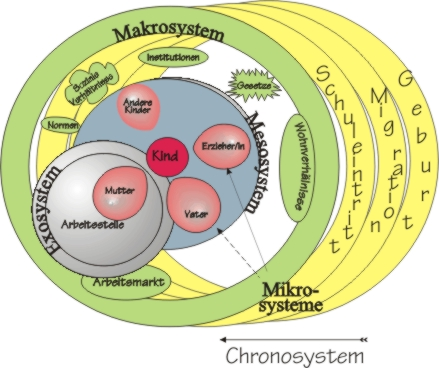
\includegraphics[scale=0.6]{figures/OekosystemBronfenbrenner}
\label{fig_bronf}
\caption{Die Systemebenen des Ökosystems bei Bronfenbrenner (\href{https://de.wikipedia.org/wiki/Datei:\%C3\%96kosystemBronfenbrenner.jpg}{Wikipedia.org}, unter GNU-FDL CC BY-SA 3.0).}
\end{figure}

 \begin{quote}
Ein Mikrosystem ist ein Muster von Tätigkeiten und Aktivitäten, Rollen und zwischen-menschlichen Beziehungen, das die in Entwicklung begriffene Person in einem gegebenen Lebensbereich mit seinen eigentümlichen physischen und materiellen Merkmalen erlebt. Ein Lebensbereich ist ein Ort, an dem Menschen leicht direkte Interaktion mit anderen aufnehmen können.  (Bronfenbrenner, 1981, S. 38)
 \end{quote}
Demnach definieren Mikrosysteme die unmittelbare Lernumwelt des sich entwickelnden Kindes. Eine Kindergartengruppe beispielsweise kann als Mikrosystem charakterisiert werden, in das Kinder und Erzieher/-innen einbezogen sind. In den meisten Fällen durchlaufen Kinder im Vorschulalter zwei Mikrosysteme, die einen bedeutsamen Einfluss auf ihre Entwicklung haben. Das sind erfahrungsgemäß zum einen die Familie und zum anderen eine Kindertageseinrichtung. Weiterführend sind die Mikrosysteme in Kontexte eingebunden, die zunehmend umfassender werden und als Meso-, Exo- und Makrosysteme bezeichnet werden\footnote{Für die vorliegende Arbeit sind nur das Mikro- und Mesosystem interessant. Diese Begriffe werden auf den folgenden Seiten ausführlicher erläutert. Auf die weiteren Systemebenen (Exo- und Makrosystem) wird im Folgenden nicht mehr eingegangen. An dieser Stelle sei lediglich auf die entsprechende Literatur verwiesen, Bronfenbrenner (1981).}. 

	"`Ein Mesosystem umfasst die Wechselbeziehungen zwischen den Lebensbereichen, an denen die sich entwickelnde Person aktiv beteiligt ist"' (Bronfenbrenner, 1981, S. 41). Zum Beispiel bildet die Wechselbeziehung zwischen einer Kindertageseinrichtung und einer Familie ein Mesosystem. Nach Bron\-fen\-bre\-nner wird eine intensive Beziehung zwischen Familie und Kindertageseinrichtung als positiv für die kindliche Entwicklung angesehen. Die Entwicklungsbedingungen sind am ungünstigsten, wenn das Mesosystem schwach verbunden ist oder gar keine Wechselbeziehung zwischen den Mikrosystemen besteht. Umgekehrt wird das entwicklungsfördernde Potential eines Lebensbereichs gesteigert, wenn die unterstützenden Verbindungen zwischen den Mikrosystemen durch Personen hergestellt werden, mit denen das sich entwickelnde Kind Primärdyaden gebildet hat, z.B. die Mutter und die Erzieher/-innen als Erziehungspartner (Bronfenbrenner, 1981, S. 205). Wenn ein Konflikt im Miteinander zwischen den Personen entsteht, die an der Entwicklung eines Kindes beteiligt sind, führt dies zu einer enormen Belastung für das Kind. Seine Entwicklung in der Familie, im Kindergarten oder in der Schule wird dann begünstigt, wenn in beide Richtungen offene Kommunikation besteht. 
	
Bronfenbrenner betont zudem: "`Das entwicklungsfördernde Potenzial von Lebensbereichen ist umso größer, je persönlicher die Kommunikation zwischen ihnen ist"' (Bronfenbrenner, 1981, S. 207). Neben der Wichtigkeit der Kommunikation im regulären Alltag hängen laut Griebel (2010) besonders die Über\-gangs\-kompe\-ten\-zen, d.h. die Möglichkeiten und der Willen, den Übergang erfolgreich zu bewältigen, von der Fähigkeit und Bereitschaft aller Beteiligten zu Kommunikation und Partizipation ab (Griebel, 2010, S. 4). Das entwicklungsfördernde Potential eines Lebensbereichs (z.B. Kindertageseinrichtung) in einem Mesosystem wird weiterhin gesteigert, wenn ein Kind den ersten Übergang in diesen Lebensbereich nicht alleine, sondern in Begleitung seiner Bezugspersonen durchläuft. Ferner werden die Übergangssituationen erheblich erleichtert, wenn sowohl die Familie als auch die Kindertageseinrichtung bereits vor dem Übergang  (z.B. vor der Aufnahme in den Kindergarten oder in die Schule) über einschlägige Informationen, Beratungsangebote und Erfahrungen verfügen (Bronfenbrenner, 1981, S. 208).

	Bronfenbrenner hebt in seiner sozial-ökologischen Theorie also die Notwendigkeit einer engen Zusammenarbeit zwischen den Familien und Kindertageseinrichtungen im Interesse der Kinder heraus. Sie zeigt besondere Relevanz einer intensiven gemeinsamen Gestaltung der Umwelt und der bewussten, klaren Absprachen bei den Übergängen auf. Nach Bronfenbrenner verlaufen Entwicklungsprozesse umso erfolgreicher, je besser die verschiedenen Mikro- und Mesosysteme miteinander verbunden sind und aufeinander abgestimmt sind. Laut Thiersch gilt dieses Argument umso stärker, je jünger die Kinder sind (Thiersch, 2006, S. 86). Zum ähnlichen Ergebnis kommen Sandberg und Vuorinen (2008). Sie stellten im Rahmen ihrer Studie fest: je jünger die Kinder, desto wichtiger ist der tägliche Kontakt zwischen Eltern und pädagogischen Fachkräften. Mit zunehmenden Alter der Kinder verlor die Zusammenarbeit mit den Eltern jedoch an Bedeutung (Sandberg \& Tuula, 2008, S. 151-161).
	
	Dem sozial-ökologischen Modell zufolge sind Kindertageseinrichtung und Familie zwei Systeme bzw. Umwelten, in denen Kinder aufwachsen und unterschiedliche Erfahrungen machen. Sie beeinflussen und ergänzen sich gegenseitig. Darum ist es wichtig, dass diese beiden Umwelten miteinander kooperieren, um die bestmögliche Entwicklung und Förderung des Kindes zu ermöglichen und zu unterstützen. 
	
Die Theorie von Bronfenbrenner steht somit im Einklang mit den Ergebnissen von den in vorausgehenden Abschnitten vorgestellten Untersuchungen und Förderprojekten, die die Notwendigkeit der Erziehungs- und Bildungspartnerschaft zwischen Erzieher/-innen und Eltern sowohl aus der Perspektive der Einrichtung als auch aus der Perspektive der Kinder und der Eltern hervorheben. 

Die bisherigen Ausführungen haben verdeutlicht, dass der gestiegene Stellenwert der Zusammenarbeit zwischen pädagogischen Fachkräften und Eltern in den letzten Jahrzehnten auf unterschiedliche Gründe zurückzuführen ist.

\section{Empirische Forschungsergebnisse}  
Das vorliegende Kapitel widmet sich den empirischen Befunden zum Thema "`Bil\-dungs- und Erziehungspartnerschaft in den Kindertageseinrichtungen"' sowohl auf der nationalen als auch auf der internationalen Ebene. Die Recherche hat ergeben, dass sich insgesamt nur wenige empirische Studien in diesem Bereich finden. Dies betrifft insbesondere den deutschsprachigen Raum. Die meisten Studien sind entweder wenig aktuell, d.h. sie wurden hauptsächlich im Zeitraum von 1980 bis 2002 durchgeführt oder enthalten zu kleine Stichproben bzw. sind thematisch sehr eng angelegt. Auch zu der Umsetzung der Rahmenrichtlinien der Bundesländer in den Kindergärten sowie zur Wirksamkeit unterschiedlicher Formen der Elternarbeit gibt es so gut wie keine aktuellen Untersuchungen.

	Was die Effekte einer aktiven Zusammenarbeit zwischen Fachkräften und Eltern auf die Entwicklung der Kinder betrifft, wurden diese bislang wenig erforscht. Im deutschsprachigen Raum gibt es kaum Längsschnittuntersuchungen, die diese Frage beantworten könnten. In Anbetracht dessen, dass die Entwicklung der Kinder von zahlreichen Faktoren beeinflusst wird, überrascht das jedoch nicht. Mögliche Effekte einer Zusammenarbeit zwischen Eltern und pädagogischen Fachkräften lassen sich empirisch nur schwer nachweisen. Dennoch liefern einige Studien, vor allem aus den USA, Belege für den positiven Effekt eines Besuchs von Familien unterstützenden Institutionen. Wie beispielsweise die im Abschnitt 4.3 erwähnten \textit{"`Perry Preschool Project"', "`Effective Provision of Pre-School"'} (EPPE) sowie die Hamburger Sprachentwicklungslängsschnittstudien.
	
Im Rahmen der internationalen Forschung liegen zwar diverse Studien zu diesem Thema vor, allerdings wurden die meisten davon innerhalb von Modellprojekten bzw. gezielten Förderprogrammen durchgeführt. Außerdem haben die Studien vorwiegend einen zeitlich befristeten Projektcharakter und nur wenige der Projekte sind wirklich evaluiert. Zudem beschäftigen sich die meisten Untersuchungen kaum mit der Zusammenarbeit mit Familien im regulären Kindergartenalltag.

Im Folgenden werden einige der wichtigsten und aktuellsten Studien vorgestellt.

\subsection{Erwartungen der Eltern an die Zusammenarbeit mit Kindertageseinrichtungen} 
Eine der wichtigsten Erwartungen der Eltern an die Kindertageseinrichtungen ist ein offener, regelmäßiger Austausch sowohl über die Entwicklung und Verhaltensweisen ihres Kindes als auch über für sie relevanten pädagogischen Themen sowie allgemeinen Kindergartenangelegenheiten. Insbesondere sind die informellen täglichen Kontakte wie Tür- und Angelgespräche von Bedeutung. Bei diesem informellen Austausch fühlen sich die Eltern weniger unter Druck gesetzt als bei den offiziellen Gesprächen und mehr in ihrer Elternrolle gestärkt und respektiert (OECD, 2000, S. 54). Daher nehmen sie die Möglichkeit zum täglichen Austausch gerne wahr. Laut der Studie von Fröhlich-Gildhoff, Kraus und Rönnau (2006) sind für 80\% von 1147 befragten Eltern die pädagogischen Fachkräfte nach den (Ehe-) Partner/-innen die zweit wichtigsten Ansprechpersonen in Erziehungsfragen (Fröhlich-Gildhoff et al., 2006, S. 10).
	
Weiterhin haben 30\% der Eltern in der Studie "`Hürdenlauf zur Kita"' eine unzufriedenstellende Zusammenarbeit der Einrichtungen mit den Familien als eine der qualitativen Hürden für die außerfamiliäre Betreuung angegeben. Die Eltern hätten mehr Anreize, ihr Kind in der Krippe anzumelden, wenn eine engere und intensivere Zusammenarbeit der Erzieher/-innen mit den Eltern gegeben wäre. Zum Beispiel wünschen sich die Eltern eine hochwertigere Qualität der Angebote sowohl für die Kinder als auch für die Familien sowie bessere Informationen darüber durch die pädagogischen Fachkräfte (Sachverständigenrat deutscher Stiftungen für Integration und Migration [SVR], 2013, S. 16). Diese Ergebnisse decken sich mit den Ergebnissen der NUBBEK-Studie (2013), die zeigten, dass für die meisten Mütter eine gute Zusammenarbeit zwischen Eltern und pädagogischen Fachkräften entscheidend ist. Insbesondere die Mütter mit Migrationshintergrund wünschen sich eine verbesserte Zusammenarbeit mit den Erzieher/-innen. Die Befunde veranschaulichen, dass ein stärker an den Be\-dürf\-nis\-sen der Eltern orientiertes Angebot sowie eine höhere Anzahl von mehrsprachigen Fachkräften in der Einrichtung viele Eltern dazu bewegen würde, ihr unter drei\-jähri\-ges Kind institutionell betreuen zu lassen~\parencite[S.~61-67]{Bensel_2013}.

Aus den Studien wird der Wunsch der Eltern nach Optimierung der Zusammenarbeit deutlich sichtbar. Eine enge Zusammenarbeit mit den Fachkräften stellt also für fast alle Mütter ein relevantes Kriterium bei der Wahl der Kindertageseinrichtung dar.


\subsection{Elternzufriedenheit und Partizipation der Eltern}
Eine Reihe von Studien, in denen Eltern und Erzieher/-innen in Einzeluntersuchungen oder gemeinsam zu ähnlichen Themen befragt wurden, kommen weitgehend übereinstimmend zu dem Ergebnis, dass Eltern zum großen Teil mit dem Kindergarten und der Zusammenarbeit mit den Einrichtungen zufrieden sind (z.B. Dippelhofer-Stiem \& Kahle, 1995; Textor, 1992). Diese Ergebnisse decken sich mit der Untersuchung von Wolf (2002), die sich auf eine Befragung in den neuen Bundesländern aus den Jahren 1997 und 2001 bezieht. Die Untersuchung zeigte, dass Eltern überwiegend mit der Zusammenarbeit zwischen den pädagogischen Fachkräften und Familien zufrieden sind und eher selten Kritik an den Erzieher/-innen ausüben sowie ihre Arbeit schätzen und unterstützen (Wolf, 2002, S. 32-34).

	Nach Einschätzung von Wolf liegt der mögliche Grund für diese hohe Zufriedenheit in der Scheu der Eltern, die Kindertageseinrichtung zu kritisieren, weil dies negative Konsequenzen für das Kind haben könnte. Beziehungsweise wollen sie die von ihnen ausgesuchte Einrichtung positiv sehen und sich deswegen auch mit einer wenig intensiven Zusammenarbeit zufrieden geben. Es gibt allerdings eine Gruppe von Eltern aus den sogenannten "`bildungsnahen"' Schichten, die oft Kritik am Kindergarten und vor allem an der Elternarbeit äußerten. Beide Kategorien der Eltern - sowohl zufriedene als auch unzufriedene - zeigten jedoch laut der Studie ein großes Interesse und Bereitschaft an der Mitarbeit in den Kindertageseinrichtungen (Wolf, 2002, S. 32-34).
	
Auch die Untersuchung von Jeske (1997) konnte weiterhin feststellen, dass die Zusammenarbeit mit der Kindertageseinrichtung ihres Kindes den meisten Eltern wichtig bzw. sehr wichtig ist. Sie sind der Meinung, dass der bessere Kontakt zu den Erzieher/-innen ihrem Kind nur zugutekommen wird. Das verstärkt die Motivation vieler Eltern, sich im Kindergartenalltag einzubringen  (Jeske, 1997, S. 63).

Nach eigenen Aussagen von aktiven Elternvertreterinnen und -vertretern sind sie jedoch eher dann bereit, sich in der Kindertageseinrichtung ihres Kindes zu involvieren, wenn sie das Gefühl haben, eine Veränderung bewirken zu können und sowohl von Fachkräften als auch von Eltern anerkannt und unterstützt zu werden (Hense, 2001, S. 43). Jedoch schneidet die elterliche Partizipation in Deutschland, im europäischen und außereuropäischen Vergleich, laut der OECD-Studie (2006), mit einem eher mittleren Grad ab (Pietsch, Ziesemer \& Fröhlich-Gildhoff, 2010, S. 15).

	 Die Erläuterung bisheriger Forschungsbefunde hat insgesamt aufgezeigt, dass Eltern überwiegend mit der Zusammenarbeit in den Kindertages-einrichtungen zufrieden sind sowie ein ausgeprägtes Interesse an der Kooperation mit dem Kindergarten zeigen. Dies gilt sowohl für die quer- als auch längsschnittlichen Befunde, die sich wie folgt zusammenfassen lassen: die Erziehungs- und Bildungspartnerschaft zwischen den Eltern und pädagogischen Fachkräften wird aus der Sicht der Eltern als sehr wichtig empfunden und von ihnen insgesamt als gut umgesetzt eingeschätzt. Zugleich jedoch äußern viele Eltern den Wunsch nach einer engeren Kooperation und intensiveren Einbindung in den Kindergartenalltag. Sie wollen mehr Informationen über ihr Kind erhalten und mehr Möglichkeiten zur Beteiligung haben.	
	 
Aus den bisher analysierten empirischen Forschungsergebnissen wird deutlich, dass die Forschungslage zum Thema "`Zusammenarbeit zwischen Familien und pädagogischen Fachkräften"' noch unbefriedigend ist. Wie bereits erwähnt, gibt es nur wenige aktuelle Untersuchungen, die sich ausschließlich mit der Ein\-schät\-zung der Zusammenarbeit in Kindertageseinrichtungen im Alltag aus der Sicht der Eltern beschäftigen. In der vorliegenden Untersuchung wird ein Versuch unternommen, diese Forschungslücke mithilfe der FRÖBEL-Elternbefragung zu verringern. Über die Zusammenarbeit zwischen den Eltern und Erzieher/-innen in den FRÖBEL-Kindertageseinrichtungen liegen bislang keine Forschungsergebnisse vor.

	Aus den dargestellten theoretischen Ausführungen und bezogen auf die herausgearbeiteten Forschungslücken lassen sich folgende Fragestellungen, die anschließend anhand der vorliegenden Daten untersucht werden, formulieren:
\begin{enumerate}

\item \textit{ Wie schätzen die Eltern die Zusammenarbeit zwischen den pädagogischen Fachkräften und Familien in den FRÖBEL-Kindertageseinrichtungen ein?}

\item \textit{Welche homogenen Dimensionen (thematische Subkategorien) lassen sich in der Subskala "`Zusammenarbeit mit Familien"' des FRÖBEL-Eltern\-frage\-bogens herausbilden?}
\end{enumerate}
Im folgenden empirischen Teil der Arbeit werden diese Fragestellungen näher untersucht.

\pagebreak
\vspace*{\fill}
\begin{Huge}
Teil II: Empirische Analysen
\end{Huge}
\vspace*{\fill}
\pagebreak


Nachdem die Relevanz und Notwendigkeit der Erziehungs- und Bildungspartnerschaft in den Kindertageseinrichtungen aufgezeigt und diskutiert wurde, wird in dem empirischen Teil der Arbeit versucht, die vorhin formulierten Fragestellungen zu beantworten. Die vorliegende explorative Datenanalyse bezieht sich auf einen Teilausschnitt der gesamten Untersuchung im Rahmen des Projekts "`FRÖBEL-Eltern- und Mitarbeiter/-innenbefragung 2013"'. Und zwar   wird speziell die Subskala "`Zusammenarbeit mit Familien"' im Elternfragebogen untersucht.

	Im ersten Abschnitt des folgenden Kapitels wird zunächst auf die Datengrundlage und die Stichprobe der vorliegenden Untersuchung näher eingegangen. Als nächstes wird das Instrument der Elternbefragung beschrieben. Im weiteren Schritt werden die Daten hinsichtlich der im vorherigen Kapitel formulierten Fragestellungen anhand von bestimmten Verfahren analysiert. Abschließend werden die Ergebnisse vorgestellt und diskutiert.
 
\section{Methodisches Vorgehen}  
\subsection{Datengrundlage und Stichprobe}
Die Datengrundlage für die vorliegende Untersuchung bilden die 2579 Elternfragebögen aus dem Projekt "`FRÖBEL-Eltern- und Mitarbeiter/-innenbefragung 2013"'. Es handelt sich hierbei um eine querschnittlich angelegte Felduntersuchung, die als Online-Befragung im Zeitraum vom 18.02.2013 bis zum 11.03.2013 stattgefunden hat. Die Befragung wurde von der Fachabteilung \textit{"`Pädagogik und Qualitätsentwicklung"'} der FRÖBEL Management GmbH - eine Abteilung des FRÖBEL e.V. - unter der Koordination von Jule Marx und Annegret Kieschnick durchgeführt. Die Zielsetzung der Befragung bestand darin, Auskunft über den Ist-Stand der pädagogischen Arbeit in den Kindertageseinrichtungen zum Zeitpunkt der Befragung geben zu können. Dieser sollte als  Ausgangspunkt und Chance für die weitere Qualitätsentwicklung in der Kinderbetreuung dienen.

	Bei der Befragung handelt es sich um eine Vollerhebung. Die Gruppe der Befragten bezog sowohl Erzieher/-innen, Leiter/-innen als auch Eltern der FRÖBEL-Kindertageseinrichtungen und FRÖBEL-Horte aller Standorte mit ein. Weil die meisten FRÖBEL-Einrichtungen nach dem Konzept "`der offenen Arbeit"' arbeiten, wurden die Eltern der Krippenkinder nicht als eine extra Befragungsgruppe differenziert, sondern in der Kindergarteneltern-Kategorie miterfasst. Insgesamt wurden 10.586 Eltern (Horte und Kindergärten zusammen) befragt. Da im Fokus der vorliegenden Arbeit speziell die Analyse der Item-Skala zur Einschätzung der Zusammenarbeit zwischen den pädagogischen Fachkräften und Eltern in den FRÖBEL-Kindertageseinrichtungen aus der Sicht der Familien steht, wurden Eltern, deren Kinder einen FRÖBEL-Hort besuchen, Leiter/-innen sowie pä\-da\-go\-gi\-sche Mitarbeiter/-innen, aus der Auswertung ausgeschlossen. Das heißt, in die Auswertung sind nur die Daten der Kindergarten-Eltern eingegangen. Daher besteht der in die Analyse einbezogene Datensatz aus 2579 (27\%) Elternfragebögen.
	
	Das Versenden der Zugangsdaten an die Kindergärten erfolgte durch eine externe Druckerei. Die Briefe mit dem Zugangscode wurden an die Eltern anonymisiert und nach dem Zufallsprinzip in den Einrichtungen verteilt, so dass zu keinem Zeitpunkt ein Rückschluss auf einzelne Personen möglich war. Eltern erhielten pro Kind einen Zugangscode, der zur einmaligen Teilnahme an der Befragung auf dem Onlineportal eines externen Anbieters berechtigte. Bei Geschwistern sollten sie für jedes Kind jeweils einen Fragebogen beantworten. Darüber hinaus wurden über die Fragebögen keine personenbezogenen Daten erhoben. Somit ist nicht bekannt, ob der Fragebogen hauptsächlich von den Müttern oder Vätern oder von beiden Elternteilen zusammen bzw. von der Mutter/dem Vater mit anderen Angehörigen gemeinsam ausgefüllt wurde. Es liegen auch keine demografischen Angaben (sozioökonomischer Status, Bildung, ethnische Herkunft etc.) von den Familien vor.

\subsection{Instrument der Erhebung} 
Der Elternfragebogen wurde von den Mitarbeiter/-innen der Fachabteilung \textit{"`Pä\-da\-go\-gik und Qualitätsentwicklung"'} der FRÖBEL Management GmbH erstellt. Er besteht aus folgenden Subskalen: \textit{pädagogische Arbeit in der Einrichtung, Bilinguale Erziehung, Umgang der Erzieher/-innen mit den Kindern und Eltern, Zusammenarbeit mit Familien} und die letzte Subskala erfragt, \textit{wie gut sich die Eltern über das Kind und die Einrichtung informiert fühlen}. Die Eltern wurden gebeten, in den standardisierten und anonymisierten Fragebögen insgesamt 79 geschlossene Fragen zu beantworten und zu zwei offenen Fragen Stellung zu beziehen. Der vollständige Fragebogen ist dem Anhang Nr. xx beigefügt.

	Wie bereits ausgeführt, steht im Zentrum der Untersuchung die Einschätzung der Zusammenarbeit zwischen den pädagogischen Fachkräften und Familien aus der elterlichen Sicht. Folglich ist für die weiteren Analysen spezifisch die Subskala \textit{"`Zusammenarbeit mit Familien"'} von Bedeutung. Diese besteht aus 20 geschlossenen Fragen. Die anderen Subskalen werden außer Acht gelassen, da sie für die Fragestellung irrelevant sind.
	
	Die Items der Subskala \textit{"`Zusammenarbeit mit Familien"'} enthalten die Aussagen über Entwicklungsgespräche, Elternabende, Möglichkeiten zum Austausch über das Kind sowie über Möglichkeiten zur Partizipation in der pädagogischen Arbeit der Einrichtung und im Kindergartenalltag. Zum Beispiel lautet eins der einzuschätzenden Items wie folgt: \textit{"`Die Mitarbeiter/-innen sind immer ansprechbar für meine Anliegen"'} (siehe Angang xy, "`Elternfagebogen"`, S. 5).
	
	Die einzelnen Items konnten von den Befragten auf einer vierstufigen Skala (4 = "`stimmt völlig"', 3 = "`stimmt eher"', 2 = "`stimmt eher nicht"', 1 = "`stimmt gar nicht"') eingeschätzt werden. Zusätzlich hatten die Eltern noch die Möglichkeit "`weiß nicht"' (98 = "`weiß nicht"') zu vergeben.
	   
	Um die im Kapitel 5 formulierten Fragestellungen präzise untersuchen zu können, werden im Folgenden die deskriptiven Analyseverfahren und daraus resultierenden Ergebnisse sowie die explorative Faktorenanalyse samt den Ergebnissen vorgestellt. Die explorative Faktorenanalyse stellt dabei das zentrale Verfahren der durchgeführten Untersuchung dar. Die Auswertung der Daten erfolgt mit der Statistiksoftware R. Alle Berechnungen sind im Skript dem Anhang XY beigefügt.

\section{Ergebnisse}  
\subsection{Deskriptiv-statistische Beschreibung der Daten}

Um den ersten Eindruck über die vorliegenden empirischen Daten (20 Items der Subskala "`Zusammenarbeit mit Familien"') zu gewinnen, werden zuerst die deskriptiven Analysen durchgeführt. Die deskriptiven Statistiken (siehe Tabelle 1) haben folgendes Ergebnis gezeigt: die Bewertung der meisten erfragten Aspekte liegt aus der Sicht der Eltern auf der Item-Skala im Durchschnitt von "`stimmt eher"' bis "`stimmt völlig"'\footnote{Die Antwortmöglichkeit "`weiß nicht"' wurde aufgrund der Nominalskalierung aus der Mittelwertberechnung ausgeschlossen und in den Häufigkeiten erfasst.}. Hieraus wird deutlich, dass sich die Mehrheit der Eltern überwiegend positiv bezüglich der Zusammenarbeit zwischen pädagogischen Fachkräften und Familien in den FRÖBEL-Einrichtungen äußert. Die Items 8.4 \textit{"`Ich kann mich über die Entwicklung und das Verhalten meines Kindes mit den Erzieher/-innen austauschen"'} ($M = 3.46, SD = 0.71$) und 8.3 \textit{"`Die Einrichtungsleitung hat für mich immer ein offenes Ohr"'} ($M = 3.45, SD = 0.76$) erfahren beispielsweise in der Bewertung der Eltern die höchste Zustimmung. Den niedrigsten Mittelwert mit $M = 2.72$ und $SD = 0.98$ weist das Item 8.7 \textit{"`Die Mitarbeiterinnen sind für mich Ansprechpartnerinnen in Erziehungsfragen"'} auf. Interessant ist der Umstand, dass das Item, welches die allgemeine Zufriedenheit der Eltern mit der Zusammenarbeit erfasst (Item 8.20): \textit{"`Alles in allem bin ich mit der Zusammenarbeit zwischen Kindergarten und Eltern zufrieden"'} von den Eltern trotzt der relativ guten Bewertung der meisten Items mit "`stimmt eher nicht"' bis "`stimmt eher"' ($M = 2.86, SD = 1.03$) eingeschätzt wurde. Insgesamt unterscheiden sich die Mittelwerte der Items jedoch nur marginal voneinander.

\begin{table}[h]
\label{tab_mean}
\caption{Einschätzungen der Zusammenarbeit zwischen pädagogischen Fachkräften und Familien durch die Eltern: Mittelwerte (M), Standardabweichungen (SD)}
\begin{tabularx}{\textwidth}{Xll}
\hline 
Items&
  M&
           SD\\\hline  
8.1 Ich bin zufrieden mit den Gesprächen mit den ErzieherInnen
      beim Bringen und Abholen                                                                                                                                                                                                             &
 3.19&  
           0.82   \\      
8.2 Die MitarbeiterInnen sind immer ansprechbar für meine   
      Anliegen                                                                                                                                                &
 3.39&
           0.74\\
8.3 Die Einrichtungsleitung hat für mich immer ein offenes Ohr &             
 3.45&
           0.76\\
8.4 Ich kann mich über die Entwicklung und das Verhalten
      meines Kindes mit den ErzieherInnen austauschen                                                                                             &
 3.46&
           0.71\\
8.5 Die ErzieherInnen informieren mich von sich aus über
      Erlebnisse und Entwicklung meines Kindes                                                                                                                                         &
 2.98&
           0.95\\
8.6 Ich bin mit den Entwicklungsgesprächen zufrieden                                          &
 3.27&
          0.86\\
8.7 Die MitarbeiterInnen sind für mich AnsprechpartnerInnen in             
      Erziehungsfragen                                                                                   &
 2.72&
          0.98\\
8.8 Ich merke, dass den ErzieherInnen der Austausch mit mir zu
      Erziehungsfragen wichtig ist                                                                 &
 2.74&
          1.00\\
8.9 Wenn es meine Zeit erlaubt, halte ich mich gerne für eine
      gewisse Zeit in der Einrichtung auf                                                                                                                  &
 3.21&
          0.82\\
8.10 Als Eltern haben wir ausreichend Möglichkeiten mitzuwirken                                                                                                                                                                                                                                                     &
 3.18&
          0.82\\
8.11 Eltern können sich durch ehrenamtliche Tätigkeiten in die
        pädagogische Arbeit einbringen                                                                                                                                                                                            &
 3.31&
          0.80 \\ 
8.12 Ich fühle mich willkommen, in der Einrichtung zu hospitieren   &      
 3.09&
          0.87\\
8.13 Die ErzieherInnen machen ihre pädagogische Arbeit gegenüber
        den Eltern transparent                                                                                                                                                                                                                                            &
 3.07&
          0.84\\
8.14 Die ErzieherInnen interessieren sich für meine Einschätzung
        ihrer Arbeit  &
 2.79&
          0.95\\
8.15 Die MitarbeiterInnen nehmen meine Beschwerden ernst                                                                                                        &
 3.26&
          0.77\\
8.16 Wichtige Entscheidungen werden zusammen mit den Eltern
        getroffen                                                                                                &
 3.10&
          0.91\\
8.17 Ich bin mit den Elternabenden zufrieden                                              &
 3.18&
          0.81\\
8.18 Im Rahmen der Elternabende erhalte ich wichtige    
        Informationen zu pädagogischen Themen                                                                    &
 3.15&
          0.81\\
8.19 Bei Elternabenden habe ich ausreichend Möglichkeiten mich    
        zu beteiligen                                                                                 &
 3.35&
          0.76\\
8.20 Alles in allem bin ich mit der Zusammenarbeit zwischen  
        Kindergarten und Eltern zufrieden&
 2.86&
          1.03\\
\hline 
\end{tabularx} 
\end{table}
\FloatBarrier

\subsection{Häufigkeiten} 

Im Folgenden werden einige ausgewählte Häufigkeitsergebnisse präsentiert. Die Auswahl der Items, die in diesem Abschnitt vorgestellt wird, wurde aufgrund der vorherigen theoretischen Ausführungen und der aktuellen Forschungslage zum Thema "`Erziehungs- und Bildungspartnerschaft in den Kindertageseinrichtungen"' getroffen. Dabei stehen die Items im Fokus, die sich am meisten entweder durch ihre sehr hohe oder niedrige Werte von den anderen Items abheben. In diesem Abschnitt wird veranschaulicht, wie folgende für die Gestaltung einer erfolgreichen Erziehungspartnerschaft wichtige Ansätze wie der wechselseitige kontinuierliche Austausch, Transparenz, Informationen sowie Einbeziehung der Eltern in das Kindergartengeschehen in den FRÖBEL-Kindertageseinrichtungen umgesetzt werden.

	Um eine bessere Übersicht zu gewinnen, werden im Weiteren bei der Darstellung der Ergebnisse die vier Antwortmöglichkeiten: "`stimmt gar nicht"', "`stimmt eher nicht"', "`stimmt eher"' und "`stimmt völlig"' in zwei Kategorien zusammengefasst ("`stimmt gar nicht/stimmt eher nicht"' und "`stimmt eher/stimmt völlig"'). Die vollständige Häufigkeitstabelle wird im Angang xy dargestellt.
	
	Prozentual lässt sich das Ergebnis folgendermaßen beschreiben: 89,8\% der Eltern können sich über die Entwicklung ihres Kindes mit den Erzieher/-innen austauschen (Item 8.4). 9.6\% der Eltern sagen, dass dies nicht der Fall ist und  0.6\% haben diesen Aspekt mit "`weiß nicht"' eingeschätzt.  Inwiefern die Eltern mit dem Entwicklungsaustausch zufrieden sind, konnte das Item 8.6 \textit{"`Ich bin mit den Entwicklungsgesprächen zufrieden"'} zeigen. Hier sieht die Verteilung der Antworten etwas anders als beim vorherigen Item aus. Fast 73\% der Eltern sind mit den Entwicklungsgesprächen zufrieden, 15\% stimmen der Aussage nicht oder eher nicht zu. Weitere 13\% wissen nicht, ob sie mit den Entwicklungsgesprächen zufrieden sind. Das Item 8.3 \textit{"`Die Einrichtungsleitung hat für mich immer ein offenes Ohr"'} wurde von den Eltern positiv bewertet. Circa 85\% der Eltern stimmten der Aussage zu, 9.3\% äußerten Kritik diesbezüglich und 6.1\% bewerteten das Item mit "`weiß nicht"'. Beim Bringen und Abholen der Kinder (Item 8.1) sind die meisten Eltern (81.3\%) mit Gesprächen zufrieden und 18.5\% sind unzufrieden. 88.4\% gaben an, dass die Mitarbeiter/-innen immer ansprechbar für ihre Anliegen sind (Item 8.2). Lediglich 11.3\% stimmten dem nicht zu. Bei dem Item 8.7 \textit{"`Die MitarbeiterInnen sind für mich AnsprechpartnerInnen in Erziehungsfragen"'} fiel die Bewertung im Vergleich zu oben genannten Beispielen wesentlich niedriger aus. So sehen nur 55\% der Befragten pädagogische Mitarbeiter/-innen als Ansprechpartner/-innen in Erziehungsfragen. Für 40.2\% trifft die Aussage nicht zu. 4.9\% bewerteten das Item mit "`weiß nicht"'.
	
	Bezüglich der Möglichkeit zur Beteiligung der Eltern an der pädagogischen Arbeit durch die ehrenamtlichen Tätigkeiten (Item 8.11) gaben 71\% der Eltern an, dass sie diese Möglichkeit haben. 16\% der Befragten wissen jedoch nicht, ob ihnen eine solche Möglichkeit geboten wird ("`weiß nicht"'). 
		
	Was das Willkommensgefühl der Eltern zur Hospitation in der Einrichtung ihres Kindes anbelangt (Item 8.12), stuften rund 58\% der Eltern das Item positiv ein. 17\% haben dieses Gefühl eher nicht. Ein Viertel der Eltern hat diesen Aspekt mit "`weiß nicht"' beantwortet. Dies kann im Verhältnis zu der Bewertung aller anderen Items auf dieser Stufe ("`weiß nicht"') als ein ziemlich hoher Anteil betrachtet werden. 82\% haben dabei angegeben, dass sie sich gerne für eine gewisse Zeit in der Einrichtung aufhalten würden, wenn es ihnen ihre Zeit erlaubt (Item 8.9).
	
	Inwiefern Erzieher/-innen ihre pädagogische Arbeit gegenüber den Eltern transparent machen, konnte anhand des Items 8.13 \textit{"`Die Erzieherinnen machen ihre pädagogische Arbeit gegenüber den Eltern transparent"'} erfasst werden. Ungefähr 74\% gaben an, dass die pädagogische Arbeit in der Einrichtung transparent gemacht wird. Demgegenüber fanden 22\% der Eltern die pädagogische Arbeit "`eher nicht"' oder "`gar nicht"' transparent.
	
	Inwieweit die Beschwerden der Eltern von den Mitarbeiter/-innen laut der Befragungsergebnissen ernst genommen werden, konnte man anhand des Items 8.15 \textit{"`Die Mitarbeiter/-innen nehmen meine Beschwerden ernst"'} feststellen. Das Item schätzten die meisten Eltern (74\%) positiv ein. Immer noch 12\% sagen, dass ihre Beschwerden von den Mitarbeiter/-innen nicht ernst genommen werden. Auch bei diesem Item wählten einige Eltern (fast 14\%) die Antwortmöglichkeit "`weiß nicht"'.
	
	Weiterhin wäre es noch wichtig anzumerken, dass auch beim Item 8.14 \textit{"`Die Erzieher/-innen interessieren sich für meine Einschätzung ihrer Arbeit"'} fast 21\% der Befragten diese Aussage mit "`weiß nicht"' eingeschätzt haben. Dieses Ergebnis könnte auf unterschiedliche Gründe zurückgeführt werden. Näher wird darauf in der Diskussion (Kapitel 8) eingegangen.
	
 	Alles in allem sind knapp 85\% der Eltern mit der Zusammenarbeit zwischen den FRÖBEL-Kindergärten und den Familien zufrieden (Item 8.20). Ca. 13\% sind mit der Zusammenarbeit eher unzufrieden und nur 2\% haben dieses Item mit "`weiß nicht"' beantwortet.
 	
	In der Abbildung~\ref{fig_freq} werden die ermittelten Häufigkeiten zur besseren Übersicht  grafisch dargestellt.

\begin{figure}[h]
\centering
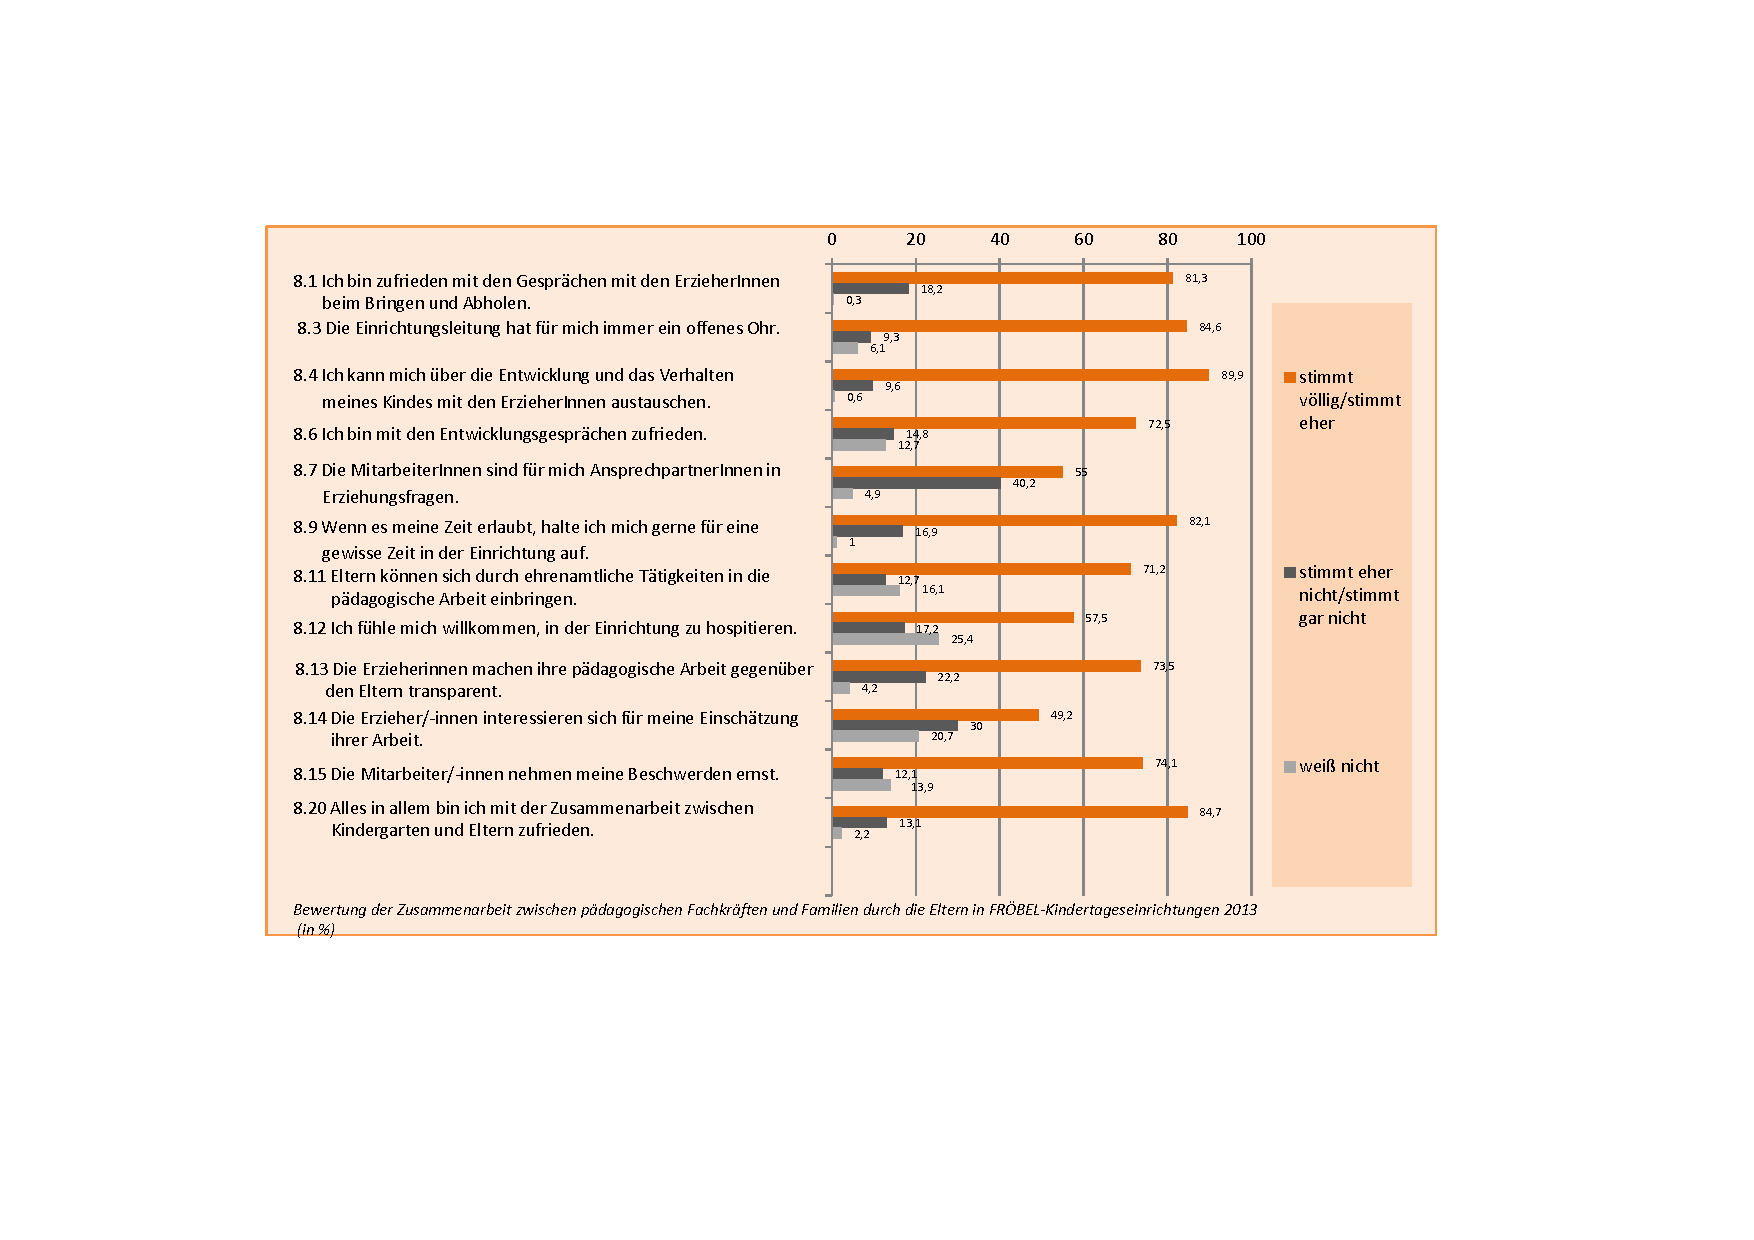
\includegraphics[scale=0.65]{figures/freq_dist3}
\caption{Bewertung der Zusammenarbeit zwischen pädagogischen Fachkräften und Familien durch die Eltern in FRÖBEL-Kindertageseinrichtungen 2013 (in \%).}
\label{fig_freq}
\end{figure}
\FloatBarrier
Die Häufigkeitsergebnisse zeigen, dass die Mehrheit der Antworten der Eltern im Bereich "`stimmt eher/stimmt völlig"' liegen. Es gibt zugleich einen Anteil der Eltern, die ihre Bewertung auf der Stufe "`stimmt eher nicht/stimmt eher"' vornehmen (max. liegt dieser Anteil bei 28.83\%). Bei einigen Items fällt interessanterweise relativ hoher Prozentsatz bei der Antwortmöglichkeit "`weiß nicht"' auf. Die möglichen Gründe für solche Bewertung der Eltern werden genauer im späteren Verlauf der Arbeit erläutert.

\subsection{Korrelationsanalyse}  
Nachdem die Mittelwerte und die Häufigkeiten vorgestellt wurden, wird im Weiteren eine Korrelationsanalyse berechnet, um herauszufinden, inwiefern die einzelnen Variablen zusammenhängen. Die Zusammenhänge zwischen den Items sind für die weitere Durchführung der Faktorenanalyse, die das zentrale Analyseverfahren des empirischen Teils darstellt, ausschlaggebend. Die Ergebnisse der Korrelationsmatrix sind dem Anhang xy beigefügt.

	Die Korrelationsmatrix zeigt, dass teilweise schwache von $r = .25$ bis starke von $r = .80$ Korrelationen zwischen den Variablen existieren. Insgesamt weisen die meisten Korrelationen einen mittleren bis hohen Zusammenhang auf. Selbst die schwachen Korrelationen sind mit $p < .000$ höchst signifikant. Hier muss allerdings angemerkt werden, dass die hohe Signifikanz ($p < .000$) aufgrund der Größe der Stichprobe ($N= 2.579$) zustande kommt. Die höchste Korrelation mit $r = .80, p < .000$ zeigen die Variablen 8.7 und 8.8, in denen die Wichtigkeit des Austausches zwischen den Erzieher/-innen und Eltern zu Erziehungsfragen thematisiert wird. Die Variablen 8.11 \textit{"`Eltern können sich durch ehrenamtliche Tätigkeiten in die pädagogische Arbeit einbringen"'} und 8.9 \textit{"`Wenn es meine Zeit erlaubt, halte ich mich gerne für eine gewisse Zeit in der Einrichtung auf"'} weisen hingegen den geringsten Zusammenhang mit allen anderen Variablen auf. Die Korrelationen von diesen beiden Items mit den anderen Items reichen von $r = .25$ bis $r = .61$.
	
	Das Ergebnis der vorgenommenen Korrelationsanalyse - signifikante mittlere bis hohe Zusammenhänge - bildet eine gute Grundlage für die Durchführung einer Faktorenanalyse, die im nächsten Kapitel vorgestellt wird.

\subsection{Exploratorische Faktorenanalyse} 
In diesem Kapitel wird die Fragestellung \textit{"`Welche homogenen Dimensionen  (thematische Subkategorien) lassen sich in der Itemskala "`Zusammenarbeit mit Familien"' herausbilden?"'} mittels einer exploratorischen Faktorenanalyse (EFA) untersucht.

	Die Grundidee der EFA ist die Datenreduktion. Es wird versucht, möglichst viele Informationen aus den ursprünglichen Daten durch eine kleinere Anzahl von Faktoren zu beschreiben. Weiterhin verfolgt die EFA das Ziel, Zusammenhänge zwischen Items auf latente Variablen zurückzuführen (Bühner, 2006, S. 180).
	
	Da der vorliegenden Untersuchung a priori kein theoretisch bzw. empirisch gut fundiertes Modell über mögliche hypothetische Faktoren zugrunde liegt, wird anhand der EFA, speziell mit der Methode der Hauptkomponentenanalyse (Principle Component Analysis, PCA) eine explorative Ermittlung der Datenstruktur unternommen. Dabei werden 19 Variablen in eine kleinere Anzahl transformiert und zu einem oder mehreren Faktoren zusammengefasst. Dies ermöglicht, die homogenen Teilbereiche auszudifferenzieren und eine übersichtliche Datenstruktur zu schaffen. Dadurch, dass der Item 8.20 \textit{"`Alles in allem bin ich mit der Zusammenarbeit zwischen Kindergarten und Eltern zufrieden"'} allgemeine Zufriedenheit und nicht wie alle anderen Items einen spezifischen Aspekt erfasst, wird er aus der Analyse ausgeschlossen. Dadurch soll die Gefahr der Datenverzerrung reduziert werden.

\subsubsection{Überprüfung der Dateneignung für eine Faktorenanalyse} 

Bevor ein faktorenanalytisches Modell spezifiziert wird, wird zunächst mittels der Korrelationsanalyse die Eignung der Daten für die exploratorische Faktorenanalyse überprüft. Der Abschnitt 7.3 "`Korrelationsanalyse"' konnte bereits zeigen, dass alle Items mittlere bis hohe Zusammenhänge aufweisen und sich somit gut für die EFA eignen. Weitere wichtige Tests zur Überprüfung der Dateneignung für die EFA sind der \textit{KMO-Test}, der Anhaltspunkte gibt, ob die Itemauswahl für die exploratorische Faktorenanalyse verwendbar ist und der \textit{Barlett-Test auf Sphärizität}, der überprüft, ob Korrelationen zwischen den Items ausreichend stark sind. In der Tabelle 2 werden die Indizien von beiden Tests dargestellt.


\begin{table}
\centering
\caption{KMO und Barlett-Test Koeffizienten}
\label{tab_KMO}
\begin{tabular}{lcl}
\hline 
\multicolumn{3}{c}{KMO and Barlett's Test} \\ 
\hline 
\multicolumn{2}{l}{Kaiser-Meyer-Olkin Measure of Sampling Adequancy } &   $0.96$ \\ 

&      Approx. Chi-Square                  &  $826.3404$ \\ 

Barlett's Test of Sphericity  &   df  & $18$ \\ 

  &   p-value                         &  $< 2.2e-16 $ \\ 
\hline 
\end{tabular} 

\end{table}

Der hohe Wert des \textit{KMO-Index} ($.96$) weist auf eine sehr gute Eignung der Daten für die Hauptkomponentenanalyse hin. Analog zum \textit{KMO-Koeffizienten} zeigt der \textit{Barlett-Test} ein hochsignifikantes Ergebnis ($p < 2.2e-16$), was bedeutet, dass alle Korrelationen größer Null und demzufolge für die PCA gut geeignet sind. Auch die Stichprobengröße ($N = 2579$) erfüllt die Voraussetzung für die Anwendung der exlporatorischen Faktorenanalyse. Denn um eine EFA durchführen zu können, muss eine Stichprobe mindestens so viele Personen umfassen, wie beobachtete Variablen vorliegen (Eid, Gollwitzer \& Schmitt, 2013, S. 918). Somit konnte die perfekte Eignung der Items für die Durchführung der EFA bestätigt werden.

\subsubsection{Methoden der Faktorenextraktion}
Im nächsten Schritt wird entschieden, wie viele Faktoren erforderlich sind, um die Datenstruktur der Subskala "`Zusammenarbeit mit Familien"' am besten abzubilden. Zur Verfügung stehen verschiedene Extraktionsmethoden, anhand derer abgeschätzt werden kann, wie viele Faktoren zu extrahieren sind. Da die Anzahl der zu extrahierenden Komponenten bei der Hauptkomponentenanalyse nicht von vornherein bekannt ist, werden in der vorliegenden Arbeit mehrere Extraktionskriterien gleichzeitig verwendet, um die optimale Anzahl der Faktoren zu bestimmen. Ein weiterer Grund für die Anwendung mehrerer Bestimmungsmethoden ist die kontroverse Diskussion bezüglich der Objektivität aller Extraktionskriterien. Dieser Diskussion zufolge ist keines von diesen Kriterien in der Lage, die Anzahl der relevanten Faktoren zuverlässig festzustellen. Zudem gibt es zur Faktorenextraktion keine allgemein verbindlichen Bestimmungen. Deshalb werden oft zur Festlegung der Anzahl der benötigten Faktoren neben den Extraktionsmethoden noch weitere Kriterien herangezogen.

	Um die optimale Anzahl der Faktoren in der vorliegenden Hauptkomponentenanalyse festzustellen, werden der \textit{Scree-Test} nach Cattell, die \textit{Parallelanalyse} nach Horn, die \textit{Very Simple Structure-Methode (VSS)} und der \textit{Minimum-Avarage-Partial-Test (MAP)} angewandt. Aufgrund der starken Kritik am \textit{Kaiser-Kriterium} wurde dieses bei der Bestimmung der Hauptkomponenten nicht berücksichtigt. Die Kritik bezog sich auf die Festlegung der Grenze von $>1$ und die Ergebnisse bisheriger Studien, die gezeigt haben, dass dieses Kriterium als Extraktionsmethode in den meisten Fällen ungeeignet ist (Fabriger et.al 1999; zitiert nach Eid et al., 2013, S. 913).
	
	Im Folgenden wird die Durchführung der ausgewählten Extraktionsmethoden samt den gewonnenen Ergebnissen beschrieben. Zuerst wurde der \textit{Scree-Plot} analysiert. Hier wurde geschaut, an welcher Stelle ein bedeutsamer Eigenwertabfall vorkommt und in der Regel nur die Eigenwerte vor dem Knick mitgezählt. In der unten stehenden Abbildung~\ref{fig_scree} ist ein Knick zwischen dem ersten und dem zweiten Eigenwert zu erkennen. Der zweite Faktor weist einen deutlich kleineren Eigenwert auf als der erste. Die restlichen Eigenwerte verlaufen ab dem zweiten Faktor gleichmäßig flach hin zu der $X$-Achse.
	
\begin{figure}[h]
\centering
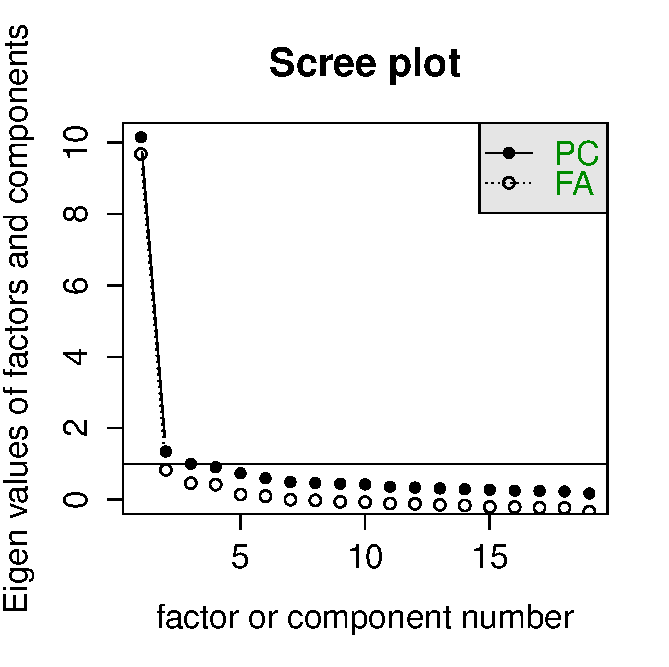
\includegraphics[scale=1]{../R-Berechnungen/Rplot.pdf}
\caption{Scree-Plot (In der Legende sind die Eigenwertverläufe der Hauptkomponentenanalyse (PC) sowie der Faktorenanalyse (FA) dargestellt).}
\label{fig_scree}
\end{figure}
									
Aus dem \textit{Scree-Plot} wird deutlich, dass es möglich wäre, entweder eine oder zwei Komponenten zu extrahieren. Somit liefert der Test keine eindeutige Lösung, denn für die weiteren Analysen ist ein klares Ergebnis erforderlich.

	Deswegen wurde als weitere Hilfe zur Bestimmung der relevanten Hauptkomponenten die \textit{Parallelanalyse} nach Horn hinzugezogen. Nach Bühner gilt diese als die beste Extraktionsmethode und sollte den anderen Methoden vorgezogen werden. Bei der durchgeführten \textit{Parallelanalyse} wurden die beobachteten Eigenwerte mit den Eigenwerten verglichen, die bei einer Faktorenanalyse mit Zufallsdaten erwartet werden. Es wurden dann nur die Faktoren extrahiert, deren Eigenwerte größer sind als die zufälligen Eigenwerte. Das Ergebnis der vorgenommenen \textit{Parallelanalyse} ist mit dem Ergebnis des \textit{Scree-Plot-Tests} identisch: man könnte entweder einen oder zwei Faktoren zur Extraktion festlegen (siehe Abbildung~\ref{fig_para}). Somit wurde wieder kein eindeutiges Ergebnis erzielt.

\begin{figure}[h]
\centering
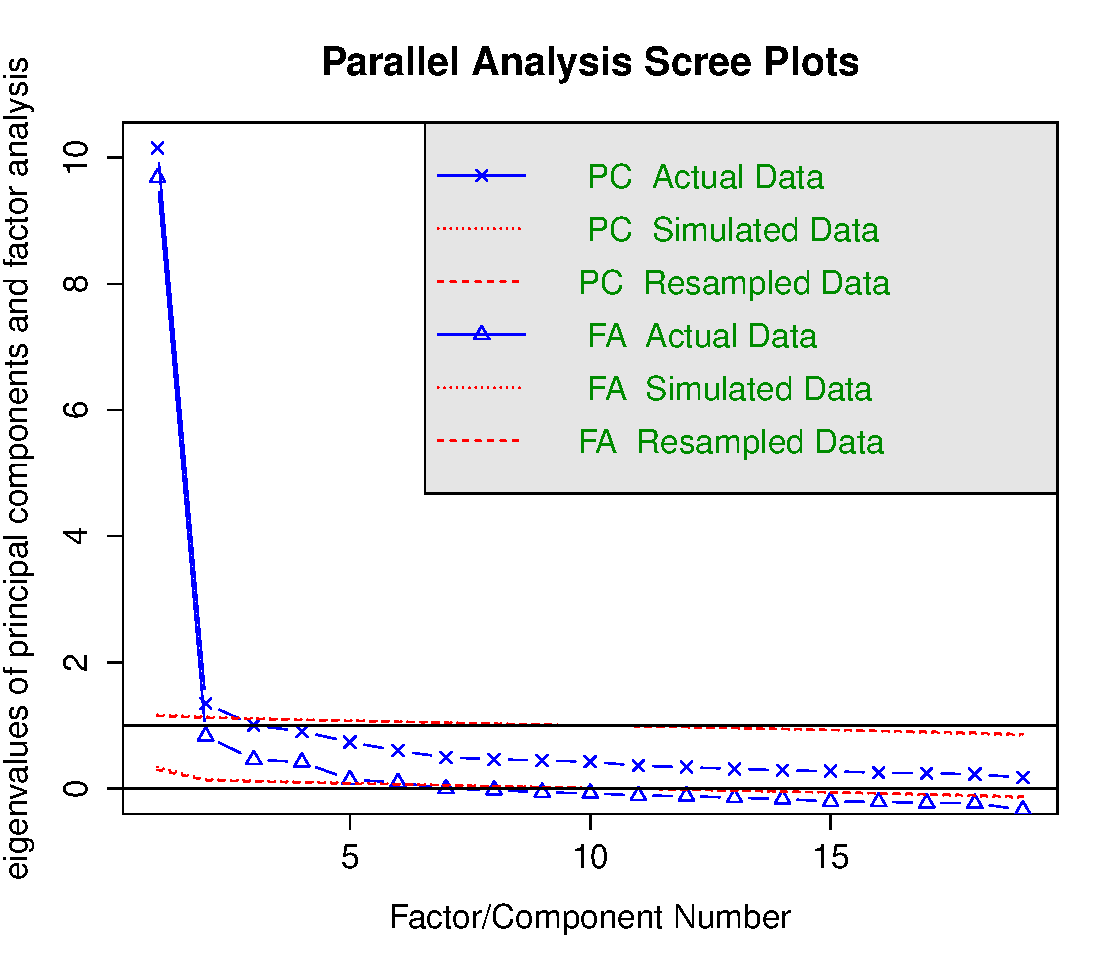
\includegraphics[scale=0.75]{../R-Berechnungen/Rplot02.pdf}
\caption{Parallelanalyse.}
\label{fig_para}
\end{figure}

Ferner wird ein weiterer Test, der \textit{Very Simple Structure-Test (VSS)}, angewandt. Er drückt aus, wie gut eine vereinfachte Faktorenmatrix die vollständige Faktorenmatrix reproduziert. Dabei können die Werte zwischen $0$ und $1$ liegen. Der Test hat folgendes ergeben:
\begin{verbatim}
	VSS (mydata, rotate="promax", fm="pc")
	Call: vss (x = x, n = n, rotate = rotate, diagonal = 
	diagonal, fm = fm, n.obs = n.obs, plot = plot, title = 
		title)
	VSS complexity 1 achieves a maximimum of 0.94 
	with 1 factors
	VSS complexity 2 achieves a maximimum of 0.7 
	with 2 factors
	\end{verbatim}
\noindent Die Komplexitätsgrade des \textit{VSS-Tests} erreicht also sein Maximum von $0.94$ mit einem Faktor und $0.7$ mit zwei Faktoren. Am besten ist die Faktorenlösung mit dem größten \textit{VSS} geeignet~\parencite[S.~274]{Quellenangaben}. Somit deuten die Ergebnisse des \textit{VSS-Tests} deutlich auf eine Ein-Faktor-Lösung hin.

	Der \textit{Minimum-Average-Partial-Test (MAP)}, zielt im Unterschied zum \textit{VSS} darauf, die durchschnittliche quadrierte Partialkorrelation zwischen den Faktoren festzustellen.  Bei diesem Test ist am besten die Faktorenlösung mit dem kleinsten \textit{MAP-Koeffizient} geeignet~\parencite[S.~274]{Quellenangaben}. Das Ergebnis dieses Tests unterscheidet sich erheblich von den Befunden der anderen Tests:
	\begin{verbatim}
	VSS (mydata,rotate="promax", fm="pc")
	The Velicer MAP achieves a minimum of 0.02 
	with 4 factors
	\end{verbatim}
\noindent Der \textit{MAP-Koeffizient} weist mit dem kleinsten Wert von $0.02$ eine Vier-Faktoren-Lösung auf, während die anderen Tests eine ein- oder zweifaktorielle Lösung festgelegt haben.

	Es wurde also gezeigt, dass es möglich wäre, entweder einen, zwei oder vier Faktoren zu extrahieren. Die unterschiedlichen Ergebnisse der vier Extraktionsmethoden führten somit zu keiner zufrieden stellenden Lösung. Daher  ist es notwendig, noch weitere Kriterien zur Bestimmung der am besten die Datenstruktur repräsentierenden Faktorenanzahl heranzuziehen. Dies wird im nächsten Abschnitt geschehen.

\subsubsection{Kriterien für die Anpassungsgüte der Modelle}
Im Folgenden werden die von den Extraktionsmethoden vorgeschlagenen Modelle mit ein-, zwei- und vierfaktoriellen Lösungen mithilfe von R und der exploratorischen Faktorenanalyse (mit Promax-Rotation) berechnet und das Ergebniss ausgegeben. Anschließend werden alle Modelle auf die Modellgüte getestet. Darauf folgend wird das Modell ausgewählt, welches am besten die Datenstruktur repräsentiert.

	Die Berechnung und die Ergebnisse der drei Modelle sind im Skript (siehe Anhang) dargestellt. An dieser Stelle werden nur die für diese Untersuchung relevanten Ergebnisse erläutert. Zunächst wird für die Beurteilung des zu testenden Modells der $\chi^2$-Anpassungstest zu Hilfe genommen. Je kleiner der $\chi^2$-Wert ist, desto besser spiegelt das Modell die tatsächlich beobachteten Daten wieder. Bei einer guten Modellpassung soll der ermittelte Testwert nicht signifikant sein. Allerdings, wie bei allen Signifikanztests, hängt auch dieser von der Größe der Stichprobe ab. "`Schon geringe Abweichungen der erwarteten von den beobachteten Varianzen und Kovarianzen können zu einer Verwerfung des Modells führen, obwohl es die Zusammenhänge zwischen den Variablen ausreichend gut beschreibt"' (Eid et al., 2013, S. 898). Dies bestätigen auch die Ergebnisse der drei untersuchten Modelle. Im Ein-Faktor-Modell fällt der Chi-Quadrat-Test mit ($\chi^2 = 6597.21, p< .000$) signifikant aus. Im Zwei- und Vier-Faktor-Modell ist der Test ebenfalls signifikant ($\chi^2  = 4761.43, p< .000;  \chi^2 = 2802.73, p < .000$).
	
	Also hat der $\chi^2$-Anpassungstest in allen drei Modellen aufgrund der sehr großen Stichprobe ($N = 2579$) ein statistisch signifikantes Ergebnis gezeigt. Das heißt, dass er sich in diesem Fall nicht optimal für die Beurteilung der Modellanpassungsgüte eignet.
	
	 Als weitere Entscheidungshilfe werden daher die Strukturkoeffizienten der Modelle analysiert. Es werden zusätzlich der Root Mean Square Error of Approximation \textit{(RMSEA)}, der Tucker-Lewis-Index \textit{(TLI)} und der Bayesian Information Criterion \textit{(BIC)} für die drei Modelle berechnet und interpretiert. Ein Modell wird dann als gut bezeichnet, wenn der \textit{RMSEA}-Wert relativ gering ist. Die Cutt-off-Werte für den \textit{RMSEA} sind bei den kleinen Stichproben ($N < 250$) $.08$ und bei den größeren Stichproben ($N > 250$) $.06.$ Der Tucker-Lewis-Index nimmt im Gegensatz zu den \textit{RMSEA} in der Regel Werte zwischen $0$ für eine schlechte Anpassung und $1$ für eine sehr gute Anpassung der Daten an. Bei \textit{TLI}$> 0.95$ ist das Modell gut an die Daten angepasst. Dieser Index wird nicht vom Stichprobenumfang beeinflusst und eignet sich im gegebenen Fall sehr gut für die Schätzung der Modellanpassungsgüte. Bei dem \textit{BIC}-Wert gilt folgendes: je kleiner der Wert, desto besser das Modell (Bühner, 2006, S. 254-259).
	 
	An dieser Stelle muss allerdings angemerkt werden, dass die Anwendung der Strukturkoeffizienten bei der exploratorischen Faktorenanalyse noch wenig untersucht ist und in der Forschungspraxis kaum praktiziert wird (Fabriger et.al 1999; zitiert nach Eid et al., 2013, S. 898).
	
	Für die drei Modelle konnten folgende Fit-Indizes erzielt werden. Das Vier-Faktor-Modell weist von den drei Modellen mit dem \textit{RMSEA} $= 0.07$, dem \textit{TLI} $= 0.94$ und dem \textit{BIC}-Index $= 470.78$ die besten Werte auf und kann als moderat bis gut bezeichnet werden. Für die zweifaktorielle Lösung wurden folgende Werte \textit{RMSEA} $= 0.11$, \textit{TLI} $= 0.85$, \textit{BIC}-Index $= 3251.8$ erreicht. Dies deutet auf keine akzeptable Modellpassung hin. Auch die Güte des einfaktoriellen Modells (\textit{RMSEA}-Index $= 0.13$, \textit{TLI} $= 0.81$ und \textit{BIC}-Wert $= 5329.11$) war nicht akzeptabel. In der folgenden Tabelle werden die Werte der Strukturkoeffizienten zusammengefasst.
\begin{table}
\caption {Fit-Indizes der Modelle mit ein-, zwei- und vierfaktoriellen Lösungen}
\label{tab_fit}
    \begin{tabular}{l|ccc}
Fit-Indizes & Ein-Faktor-Modell & Zwei-Faktor-Modell & Vier-Faktor-Modell \\ 
\hline 
 
$\chi^2$ &
             6597.21 &
     

   $4761.43$ &
    
    $2802.73$\\
    & $p < .000$ & $p < .000$ &
     $p < .000$ \\
RMSEA &
0.13 &
0.11 &
0.07\\
TLI &
0.81 &
0.85 &
0.94\\
BIC &
     5329.11 &
    3251.8 &
    470.78\\
    \hline
    \end{tabular}

    \end{table}
Anmerkungen. $\chi^2$-Anpassungstest; \textit{RMSEA}: Root Mean Square Error of Approximation, \textit{TLI}: Tucker-Lewis-Index; \textit{BIC}: Bayesian Information Criterion.


Die Analyse hat also ergeben, dass das Vier-Faktor-Modell die Datenstruktur am besten repräsentiert. Dennoch ist es bei dieser Anzahl von Items wenig sinnvoll, sich für eine vierfaktorielle Lösung zu entscheiden, da bei diesem Modell Skalen mit nur drei oder weniger Items entstehen. Das ist unter dem Gesichtspunkt der Reliabilität, selbst bei Items mit hohen Faktorladungen, zu wenig, um eine Skala gut abbilden zu können (Bühner, 2006, S. 228). Außerdem zeigen die Eigenwerte der extrahierten Faktoren, dass der erste Faktor den größten Eigenwert von $10.15$ hat, der zweite von $1.35$ –  der dritte und der vierte Faktoren weisen nur noch einen Eigenwert von $1.00$ und $0.90$ auf. Auch die Varianz der Faktoren spricht gegen ein vierfaktorielles Modell. Im Folge der Analysen ergab sich ein varianzstarker (53\%) erster Faktor, dem mit deutlichem Abstand die anderen Faktoren folgten: durch den zweiten Faktor werden 7\%, durch den dritten und vierten jeweils nur 5\% der Varianz erklärt. Somit fällt das Varianzaufklärungspotenzial von den drei anderen Faktoren im Vergleich zu dem ersten Faktor sehr gering aus. Zudem besteht im vierfaktoriellen Modell eine hohe Korrelation zwischen den Faktoren.  Die Korrelationen reichen von $.54$ bis $.68$. In Anbetracht der angeführten Argumente kann auf das Vier-Faktor-Modell verzichtet werden, obwohl die Modellgütekriterien die akzeptable Anpassung gezeigt haben. Das bedeutet, im Weiteren muss entschieden werden, welches von den übrigen Modellen (das ein- und zweifaktorielle Modell) am besten die vorliegenden Daten repräsentiert.

	Oben wurde bereits ermittelt, dass der Alpha-Koeffizient der Gesamtitemskala bei $\alpha$ $= .899$ liegt. Dieser Wert deutet ganz explizit auf eine einfaktorielle Struktur des Fragebogens hin. Genauso zeigt die starke Korrelation der Variablen, dass wenige Faktoren notwendig sind, um den ursprünglichen Informationsgehalt des Fragebogens zu erhalten. Außerdem sollte nach Bühner (2006) unabhängig von den ausgewählten Extraktionskriterien eine Anzahl von Faktoren extrahiert werden, die sich inhaltlich verständlich interpretieren lässt (Bühner, 2006, S. 202). Zudem besteht in dem Zwei- Faktor-Modell wie auch im vierfaktoriellen Modell eine hohe Korrelation zwischen den Faktoren. Die Faktoren des Zwei-Faktor-Modells korrelieren mit $r = .73$ stark miteinander. Das bedeutet, dass sie zu einem Faktor zusammengefasst werden können. Demzufolge und unter der Berücksichtigung des Grundprinzips der Hauptkomponentenanalyse und des Reliabilität-Gesichtspunktes sowie der gleichmäßig hoch untereinander korrelierenden Faktoren, wird schließlich ein Ein-Faktor-Modell gewählt.

\subsubsection{Faktorladungen}
Nachdem die Entscheidung über die Anzahl der zu extrahierenden Faktoren gefallen ist und schließlich ein Faktor extrahiert wurde, werden im weiteren Schritt die Ladungen auf dem Faktor analysiert. Die einfaktorielle Lösung ist in der Abbildung~\ref{fig_fak} dargestellt.

\begin{figure}[h]
\centering
%\includegraphics[scale=1]{../R-Berechnungen/.pdf}
\caption{Faktorstruktur der Einschätzung der Zusammenarbeit zwischen den pädagogischen Fachkräften und Familien in den FRÖBEL-Kinder\-tages\-ein\-rich\-tungen durch die Eltern.}
\label{fig_fak}
\end{figure}


8.14 Die ErzieherInnen interessieren sich für meine Einschätzung
        ihrer Arbeit                                                                                            0.82
8.8 Ich merke, dass den ErzieherInnen der Austausch mit mir zu
      Erziehungsfragen wichtig ist                                                                   0.81   
8.4 Ich kann mich über die Entwicklung und das Verhalten
      meines Kindes mit den ErzieherInnen austauschen                                0.79
8.13 Die ErzieherInnen machen ihre pädagogische Arbeit gegenüber
        den Eltern transparent                                                                            0.78
8.5 Die ErzieherInnen informieren mich von sich aus über Erlebnisse
      und Entwicklung meines Kindes                                                             0.77
8.15 Die MitarbeiterInen nehmen meine Beschwerden ernst                        0.77
8.1 Ich bin zufrieden mit der Gesprächen mit den ErzieherInnen
      beim Bringen und Abholen	                                                               0.76
8.2 Die MitarbeiterInen sind immer ansprechbar für meine Anliegen           0.75
8.16 Wichtige Entscheidungen werden zusammen mit Eltern
        getroffen                                                                                                  0.75
8.17 Ich bin mit den Elternabenden zufrieden                                                0.75
8.6 Ich bin mit den Entwicklungsgesprächen zufrieden                                 0.73  
8.7 Die MitarbeiterInnen sind für mich AnsprechpartnerInnen in             
      Erziehungsfragen                                                                                       0.73
8.18 Im Rahmen der Elternabende erhalte ich wichtige Informationen
        zu pädagogischen Themen                                                                      0.73
8.10 Als Eltern haben wir ausreichend Möglichkeiten mitzuwirken              0.71
8.12 Ich fühle mich willkommen, in der Einrichtung zu hospitieren              0.71
8.19 Bei Elternabenden habe ich ausreichend Möglichkeiten
        mich zu beteiligen                                                                                   0.70
8.3 Die Einrichtungsleitung hat für mich immer ein offenes Ohr                   0.66         
8.11 Eltern können sich durch ehrenamtliche Tätigkeiten in die
        pädagogische Arbeit einbringen                                                              0.55
8.9 Wenn es meine Zeit erlaubt, halte ich mich gerne für eine
      gewisse Zeit in der Einrichtung auf                                                          0.52

Im Prozess der Modellbildung wurden keine Items ausgeschlossen. Die Analyse der internen Konsistenz hat nicht bestätigt, dass der Ausschluss eines ltems zu einer starken Erhöhung des Chronbachs-Alpha-Wertes führen würde. Dies zeigt, dass alle Items für die Repräsentation der Information, die in den Daten vorhanden ist, wichtig sind.

	Alle Ladungen laden überwiegend gleichmäßig hoch sowie positiv auf dem Faktor. Die meisten Ladungen liegen im Bereich $a >.70$ und unterscheiden sich nur marginal voneinander. Daher kann von einer stabilen Lösung ausgegangen werden.
	
	Besonders hohes Gewicht auf dem Faktor weist das Item 8.14 \textit{"`Die Erzieher/-innen interessieren sich für meine Einschätzung ihrer Arbeit"'} mit $a= .82$ auf. Dieses zeigt die höchste Ladung, gefolgt vom Item 8.8 \textit{"`Ich merke, dass den ErzieherInnen der Austausch mit mir zu Erziehungsfragen wichtig ist"'}, welches mit $a = .81$ auf dem Faktor lädt.
	Die geringsten Ladungen weisen drei folgende Items auf: das Item 8.9 \textit{"`Wenn es meine Zeit erlaubt, halte ich mich gerne für eine gewisse Zeit in der Einrichtung auf"'} mit $a = .52$, das Item 8.11 \textit{"`Eltern können sich durch ehrenamtliche Tätigkeiten in die pädagogische Arbeit einbringen"'} mit $a = .55$ und das Item 8.3 \textit{"`Die Einrichtungsleitung hat für mich immer ein offenes Ohr"'} mit $a = .66$.   
	
	Abschließend lässt sich zusammenfassen, dass die Eltern ihre Einschätzung der Zusammenarbeit zwischen den Familien und den pädagogischen Fachkräften in den FRÖBEL-Einrichtungen auf einer Dimension vornahmen. Diese bildet verschiedene Facetten der Zusammenarbeit mit Familien ab: die Kommunikation, den Informationsaustausch über das Kind sowie die Beteiligungs- und Mitwirkungsmöglichkeiten der Eltern in den FRÖBEL-Kindertageseinrichtungen. Der gewonnene Faktor lässt sich inhaltlich am besten genauso wie die analysierte Subskala des Elternfragebogens als \textit{"`Zusammenarbeit mit Familien"'} bezeichnen und erklärt 53\% der Gesamtvarianz der untersuchten Subskala. Der Eigenwert des Faktors beträgt dabei $10.15$.
	Anschließend wurde aus den jeweiligen Items der Subskala durch Mittelwertbildung der Gesamtskalenwert gebildet. Dieser beläuft sich auf  $M = 3.2$ mit einer Standardabweichung von $SD = .49$ und weist mit dem hohen Chronbachs-Alpha-Wert von $\alpha$ $= .899$ auf eine sehr gute Reliabilität der Skala hin.
	
	Das Ergebnis der Hauptkomponentenanalyse kann als Basis für weiterführende Analysen dienen, beispielsweise für eine Regressionsanalyse.
	
An dieser Stelle soll allerdings angemerkt werden, dass in der Praxis nur selten mehrere Methoden, die in dieser Arbeit zur Bestimmung der optimalen Anzahl der Faktoren zum Einsatz gekommen sind, angewandt werden. Man verwendet meist eine, höchstens zwei Methoden. In der Regel orientiert man sich bei der Entscheidung wie viele Faktoren zu extrahieren sind, zum einen an den \textit{Scree}-Testergebnissen bzw. an dem oft kritisierten \textit{Kaiser-Kriterium} (Eigenwerte $>1$), indem die Eigenwerte der Faktoren angeschaut werden. Das Ziel der vorliegenden Untersuchung bestand neben der Beantwortung der im Kapitel 5 formulierten Fragestellungen auch darin, die unterschiedlichen Methoden der Faktorenextraktion sowie die möglichen Vorgehensweisen aufzuzeigen, wenn die Ergebnisse bei der Bestimmung der optimalen Anzahl der Faktoren nicht wunschgemäß bzw. nicht eindeutig ausfallen.

	Im folgenden Kapitel werden die wichtigsten Ergebnisse der vorliegenden Untersuchung zusammengefasst und diskutiert sowie in Verbindung mit den Befunden der bisherigen Studien zu der Thematik "`Erziehungs- und Bildungspartnerschaft zwischen den Eltern und pädagogischen Fachkräften in den Kindertageseinrichtungen"' gesetzt.

\section{Diskussion der Ergebnisse}
Neben der Aufgabe, den Lesern die Relevanz und Notwendigkeit der Erziehungs- und Bildungspartnerschaft zwischen den Familien und pädagogischen Fachkräften aufzuzeigen sowie einen Einblick in die Forschungsbefundlage zu diesem Thema zu geben, bestand das Ziel der vorliegenden Untersuchung darin, mithilfe der empirischen Analysen zu veranschaulichen, wie die Zusammenarbeit zwischen den Familien und pädagogischen Fachkräften in den FRÖBEL-Kinder\-tages\-ein\-rich\-tun\-gen aus der Perspektive der Eltern beurteilt wird.  Weiterhin wurde anhand der exploratorischen Faktorenanalyse untersucht, welche homogenen Bereiche sich in der Itemskala "`Zusammenarbeit mit Familien"' herausbilden  lassen.

	Die Ergebnisse der durchgeführten Analyse veranschaulichen, dass die meisten Eltern die Zusammenarbeit zwischen Familien und pädagogischen Fa\-chkräf\-ten in den FRÖBEL-Kindergärten grundsätzlich positiv einschätzen. Daraus wird deutlich, dass viele Aspekte der Itemskala "`Zusammenarbeit mit Familien"' in den FRÖBEL-Einrichtungen weitgehend umgesetzt werden.
	
	Insbesondere erfährt der Aspekt \textit{"`Austausch und Kommunikation"'} zwischen den pädagogischen Fachkräften und Familien, welcher auch in der Rahmenkonzeption des FRÖBEL-Trägers stark betont wird, eine große Zustimmung der Eltern. 
	
Rund 90\% der befragten Eltern haben dem Item 8.4 \textit{"`Ich kann mich über die Entwicklung und das Verhalten meines Kindes mit den Erzieher/-innen austauschen"'} zugestimmt. Mit 90\% erreicht dieses Item den höchsten Prozentwert in der Itemskala "`Zusammenarbeit mit Familien"'.
 
	Ebenso positiv wurden auch Entwicklungsgespräche von den Eltern bewertet: die große Mehrheit der Eltern (72.5\%) gab an, mit den Entwicklungsgesprächen zufrieden zu sein (Item 8.6). Somit deutet dieses Item darauf hin, dass Entwicklungsgespräche zwischen Erzieher/-innen und Eltern zu einem großen Teil in den FRÖBEL-Einrichtungen praktiziert werden. Allerdings gab es Eltern, die Entwicklungsgespräche weniger positiv bewerteten. Fast 15\% der Befragten gaben an, dass sie mit Entwicklungsgesprächen unzufrieden sind und knapp 13\% beantworteten das Item mit "`weiß nicht"'. Die Antwortvergabe "`weiß nicht"' könnte einerseits damit zusammenhängen, dass aufgrund der kurzen Besuchsdauer noch keine Entwicklungsgespräche zum Zeitpunkt der Befragung stattgefunden haben. Andererseits könnte es darauf hindeuten, dass Entwicklungsgespräche (z.B. aufgrund der ungünstigen Strukturbedingungen) in einigen Einrichtungen nur selten oder überhaupt nicht durchgeführt werden. Ein weiterer Grund dafür könnte darin liegen, dass seitens der Eltern Entwicklungsgespräche nicht wahrgenommen bzw. als unwichtig betrachtet werden. In diesem Fall sollten/könnten die Eltern durch die Erzieher/-innen für dieses Thema stärker sensibilisiert werden. Denn zu einer gelingenden Erziehungs- und Bildungspartnerschaft gehören der intensive Austausch und die Abstimmung über die weiteren Erziehungs- und Bildungsziele. Allerdings sollten    pädagogische Fachkräfte, insbesondere wenn es darum geht die kritischen Einschätzungen bezüglich des Entwicklungsstandes des Kindes an die Eltern zurückzumelden, vorsichtig sein. Laut der Ergebnissen der Studie von Gabriele Peitz (2004) charakterisieren Mütter die Erzieher/-innen oft als inkompetent, wenn sie Verhaltensauffälligkeiten bei ihrem Kind feststellen und diesbezüglich vorschnell und ungebeten Ratschläge geben (Peitz, 2004, S. 265-270).
	
	Des Weiteren berichteten 81.3\% der Eltern, dass sie mit den Gesprächen zwischen den Eltern und Erzieher/-innen beim Bringen und Abholen zufrieden sind (Item 8.1). Die restlichen fast 19\% äußerten Kritik hierzu. Vor dem Hintergrund der Ergebnisse der bisherigen Untersuchungen, die deutlich machen, dass den Tür- und Angelgesprächen in der Zusammenarbeit mit Familien ein hohes Gewicht zukommt (vor allem beim Kontaktaufbau mit den benachteiligten Familien), erscheint dieser Prozentsatz recht hoch zu sein. Ein möglicher Grund für die Unzufriedenheit der Eltern könnte sein, dass die Tür- und Angelgespräche nicht entsprechend ihren Wünschen und Vorstellungen verlaufen. An dieser Stelle wäre empfehlenswert, die individuellen Bedürfnisse und Erwartungen der Eltern bei den Tür- und Angelgesprächen noch stärker zu berücksichtigen. Da die regelmäßigen Gespräche eine Vertrauensbasis schaffen und somit die Grundlage für die gute Erziehungs- und Bildungspartnerschaft bilden.
	
Mit deutlichem Abstand zu den oben vorgestellten Items, aber bei immer noch relativ hohem Zustimmungsgrad, sehen 55\% der Eltern die Erzieher/-innen als Ansprechpartner/-innen in Erziehungsfragen: \textit{"`Die MitarbeiterInnen sind für mich AnsprechpartnerInnen in Erziehungsfragen"'}. Jedoch sieht immerhin fast die Hälfte der Eltern (40\%) das anders und schätzt diese Aussage eher als nicht zutreffend ein. Dieses Ergebnis unterscheidet sich deutlich von den bereits erwähnten Befunden der Untersuchung von Fröhlich-Gildhoff et al. (2006). Laut dieser Studie sind für 80\% der befragten Eltern die Erzieher/-innen nach den (Ehe-) Partner/-innen die wichtigsten Ansprechpersonen für Erziehungsfragen (Fröhlich-Gildhoff et al., 2006, S. 10).  

Dass der ziemlich hohe Anteil der Eltern (40\%) die Erzieher/-innen nicht als Ansprechpartner/-innen in Erziehungsfragen sehen, könnte einerseits damit zusammenhängen, dass der Erzieherberuf in unserer Gesellschaft nach wie vor, trotz einer gewissen gesellschaftlichen Tendenz zur Aufwertung, ein geringes Ansehen erfährt. Erzieher/-innen werden oft lediglich als Betreuer/-innen bzw. Aufpasser/-innen gesehen, aber wenig als professionelle pädagogische Fachkräfte anerkannt. Die fachlichen Kompetenzen der Erzieher/-innen werden immer noch von vielen in Frage gestellt. Dies ist nicht zuletzt der eigenen Haltung der Erzieher/-innen zu verdanken. Sie ist in hohem Maße dafür entscheidend, in welcher Rolle - lediglich als Aufpasser/innen und Betreuer/-innen oder als kompetente Fachkräfte und Erziehungspartner/-innen - sie von den Eltern gesehen werden. Erzieher/-innen müssen sich vermehrt ihrer eigenen Kompetenz und pädagogischen Stärken bewusst werden und davon überzeugt sein, dass ihr Handeln sinnvoll und wirksam ist und als Professionelle auf die Eltern zugehen.  
Ein weiterer Erklärungsansatz ist auf die Studie von Sturzbecher \& Bredow (1998) zurückzuführen. Sie konnten feststellen, dass die häufigen Ursachen für die Hemmungen der Eltern die Erzieher/-innen bei bestimmten Problemen bzw. Fragen anzusprechen, oft an dem Fremdheitsgefühl gegenüber den Erzieher/-innen, Fehlen von günstigen Zeitpunkten, an der Befürchtung vor negativen Folgen für das Kind sowie vor dem Einmischen der Erzieher/-innen in Familienangelegenheiten liegen (Sturzbecher \& Bredow, 1998, S. 193-233). 

	Ähnlich wie beim vorausgehenden Item schätzten fast 53\% der Eltern das Item 8.8. \textit{"`Ich merke, dass den Erzieher/-innen der Austausch mit mir zu Erziehungsfragen wichtig ist"'} positiv ein. Weitere 36\% der Befragten äußerten Kritik zu dieser Aussage und 11\% entschieden sich für die Antwort "`weiß nicht"'. An dieser Stelle sei angemerkt, dass diese beiden Items 8.7 und 8.8 die höchste Korrelation ($r = .80$) untereinander aufgewiesen haben. Daher ist es nicht erstaunlich, dass die Bewertung der Eltern ähnlich ausfällt. Inhaltlich bedeutet das, je häufiger die Eltern merken, dass den Erzieher/-innen der Austausch mit ihnen zu Erziehungsfragen wichtig ist, desto stärker nehmen sie die Erzieher/-innen als Ansprechpartner/-innen wahr. Aus diesem Grund ist es wichtig, dass die Erzieher/-innen, ihr Interesse an dem Austausch mit den Eltern verstärkt signalisieren bzw. sich um einen regelmäßigen Kontakt bemühen, wenn sie von den Eltern als Erziehungspartner/-innen in Erziehungsfragen gesehen werden wollen. Insbesondere, wenn die Er\-zieher/-innen auf die Eltern zugehen und den ersten Schritt machen, gewinnen diese den Eindruck, dass die Fachkräfte wirklich an einer Erziehungs- und Bildungspartnerschaft interessiert sind. Dies ist besonders bei den Eltern wichtig, wie die bisherigen Ausführungen gezeigt haben, die sich aufgrund der vielfältigen gesellschaftlichen Veränderungen und deren Auswirkungen auf das Familienleben zunehmend belastet und hinsichtlich ihrer Erziehungskompetenzen verunsichert fühlen.
	
	Die vorliegenden Befunde haben veranschaulicht, dass der Aspekt \textit{"`Austausch und Kommunikation"'} von den meisten Eltern positiv eingeschätzt wurde. Insbesondere dem individuellen Austausch über das einzelne Kind wurde ein hoher Stellenwert seitens der Eltern eingeräumt. Damit kann die Umsetzung der Leitlinien der Zusammenarbeit mit Familien bestätigt werden, deren zufolge der regelmäßige Dialog über die Entwicklung und die Bildungsinteressen der Kinder zu den Grundlagen der Zusammenarbeit in den FRÖBEL-Einrichtungen gehört. Allerdings gab es neben den überwiegend positiv eingeschätzten Aussagen einige Diskrepanzen in den Antworten der Eltern zu diesen Items. Dies weist darauf hin, dass im Bereich "`Austausch und Kommunikation"` noch ein gewisses Entwicklungspotenzial besteht.
	
	Ein weiterer wichtiger Aspekt für eine gelungene Erziehungs- und Bildungspartnerschaft zwischen pädagogischen Fachkräften und Eltern, welches auch in der Forschungs- sowie Praxisliteratur immer wieder betont wird, ist \textit{"`die Beteiligung"'} der Eltern am Kindergartengeschehen. Die Ergebnisse der FRÖBEL-Elternbefragung zeigen, dass die Mehrheit der Eltern (76.3\%) die Möglichkeiten zur Mitwirkung in den FRÖBEL-Einrichtungen positiv einschätzte (Item 8.10). Ferner zeigte sich ein positives Bild zu der Aussage 8.11 \textit{"`Eltern können sich durch ehrenamtliche Tätigkeiten in die pädagogische Arbeit einbringen"'}. 71\% der Eltern stimmten dieser Aussage zu. 16\% der Eltern wissen hingegen nicht, ob sie die Möglichkeit zur ehrenamtlichen Beteiligung an der pädagogischen Arbeit haben. Dies lässt zum einen die Vermutung zu, dass Eltern wenig oder gar kein Interesse an der ehrenamtlichen Tätigkeit in der Kindertageseinrichtung ihres Kindes haben und deswegen informieren sich darüber nicht. Hier darf zudem nicht außer Acht gelassen werden, dass der Zeitumfang, den die Eltern in der Kindertageseinrichtung ihres Kindes verbringen wollen und können, häufig begrenzt ist, was die Teilnahme an der ehrenamtlichen Tätigkeit nur bedingt möglich macht. In diesem Fall bleibt den pädagogischen Fachkräften dieses wenige Interesse der Eltern an der ehrenamtlichen Tätigkeit mit möglichst wertschätzender Haltung zu akzeptieren.
	
Zum anderen könnte der hohe Prozentsatz von "`weiß nicht"' Antworten darauf hindeuten, dass von der Einrichtung solche Möglichkeiten nicht angeboten werden bzw. die Eltern werden nicht ausreichend darüber informiert. Dies würde jedoch den in der FRÖBEL-Rahmenkonzeption gestellten Anforderungen an die Kindertageseinrichtungen widersprechen: "`Die Förderung ehrenamtlichen Engagements gehört [...] zum Selbstverständnis jeder FRÖBEL-Einrichtung […]"' (Kieschnick et al., 2014, S. 28). Hier gilt es ebenso wie im Falle der Entwicklungsgespräche, den Eltern aufzuzeigen und bewusst zu machen, wie wichtig es für die weitere erfolgreiche Entwicklung der Zusammenarbeit ist, sich am Bildungsort ihres Kindes zu beteiligen. Deshalb sollten Eltern zur ehrenamtlichen Mitwirkung ermutigt und unterstützt werden. Dies kann gefördert werden, indem man ihnen zum Beispiel angemessene Aufgaben zutraut und explizit anbietet. 

	Was die Hospitation anbelangt, wird in der Rahmenkonzeption des Trägers (siehe Kapitel 3) betont, dass die Eltern immer willkommen sind, in der Einrichtung zu hospitieren. Dieser Aussage stimmte über die Hälfte der Eltern (58\%) zu. 17\% gaben an, sie fühlen sich eher nicht oder gar nicht willkommen, in der Einrichtung zu hospitieren. Ein Viertel der Eltern bewertete dieses Item mit "`weiß nicht"'. In der Antwortskala "`weiß nicht"' hebt sich dieses Item mit dem größten Prozentwert von den anderen Items ab. Diese Befunde legen mehrere Erklä\-rungs\-an\-nah\-men nahe. Zum einen ist es denkbar, dass die Eltern über die Möglichkeit zur Hospitation in den Einrichtungen nicht ausreichend informiert sind. Dies kann einerseits daran liegen, dass die Eltern selbst an einer Hospitation kein Interesse haben, andererseits die Hospitation ist möglicherweise seitens des pädagogischen Personals nicht wirklich erwünscht, denn nicht jede/-r Erzieher/-in ist bereit, sich von den Eltern bei ihrer Arbeit beobachten zu lassen. Um dem Desinteresse, Informationsmangel aber auch eventueller Unsicherheit der Eltern entgegen zu wirken, sollte den Eltern verstärkt das Willkommensgefühl zur Hospitation vermittelt werden. Dadurch erhalten sie die Möglichkeit, den Alltag des eigenen Kindes mitzuerleben und aktiv zu bereichern. Damit wird Transparenz des erzieherischen Handelns geschaffen und infolgedessen die angestrebte, gesellschaftliche Anerkennung und Wertschätzung des Erzieherberufs erhöht. Dies bestätigt auch die Untersuchung von Fröhlich-Gildhoff et al. (2006). Laut den Ergebnissen dieser Studie bekamen die Eltern durch den Einbezug in die pädagogische Arbeit eine genauere Vorstellung und ein besseres Verständnis vom Kindergartenablauf. Aufgrund dessen sind der Respekt gegenüber den Erzieher/-innen sowie die eigene Beteiligung und Bereitschaft zur Unterstützung gestiegen (Fröhlich-Gildhoff et al., 2006, S. 10).
	
	Ferner gaben 68\% der Eltern an, dass die wichtigen Entscheidungen gemeinsam mit den Eltern getroffen werden (Item 8.16). 20\% der Eltern, die zu dieser Aussage Stellung bezogen haben, stimmten dem nicht zu. 12\% der Eltern konnten dieses Item weder positiv noch negativ bewerten und wählten die Antwort "`weiß nicht"'. Dies könnte eventuell damit zusammenhängen, dass der Fragebogen von einem Elternteil ausgefüllt wurde, der sich eher wenig im Kindergarten seines Kindes beteiligt und deswegen nicht weiß, ob die wichtigen Entscheidungen zusammen mit den Eltern getroffen werden bzw. erachten die Eltern selbst es nicht für notwendig, sich an den Entscheidungen der Einrichtung zu beteiligen. Was die anderen 20\% anbetrifft, die dieser Aussage nicht zustimmten, könnte dies darauf hindeuten, dass sie möglicherweise bei wichtigen Entscheidungen seitens der Einrichtung nicht gerne einbezogen werden oder die Beteiligung nicht ganz ihren Wünschen und Vorstellungen entspricht. Die festgestellte Unzufriedenheit von einem Fünftel der befragten Eltern kann man als einen Indikator betrachten, dass die im Kinder- und Jugendhilfegesetz sowie in den Bildungsplänen und in der FRÖBEL-Rahmenkonzeption geforderte elterliche Beteiligung an Entscheidungsprozessen in Kindertageseinrichtungen noch weiter ausgebaut werden könnte, falls seitens der Eltern diesbezüglich Interesse und Wunsch bestehen.
	
	Mit deutlichem Abstand zu den anderen Items zeichnet sich das Item 8.14 \textit{"`Die Erzieher/-innen interessieren sich für meine Einschätzung ihrer Arbeit"'} ab. Bei diesem Aspekt ergaben sich zudem die größten Diskrepanzen in der Bewertung der Eltern. Nur knapp die Hälfte der Eltern (49\%) stimmte der Aussage zu. Ein Drittel der Eltern behauptete, dass die pädagogischen Fachkräfte an einer Rückmeldung in Bezug auf ihre Arbeit kein Interesse zeigen und 21\% wussten nicht, ob das Interesse seitens der Erzieher/-innen bezüglich der Einschätzung ihrer Arbeit durch die Eltern besteht. 
	
Die Gründe für die sehr unterschiedliche Bewertung der Eltern können sehr vielfältig sein. Zum einen hängt das möglicherweise mit der Haltung der Erzieher/-innen zusammen: sie sind davon überzeugt, sie würden ihre Arbeit gut machen und brauchen daher kein Feedback. Zum anderen gibt es auch heute noch Fachkräfte, die die Eltern nicht als Experten ihrer Kinder anerkennen und der Auffassung sind, dass sie besser als die Eltern wissen, was das Beste für das Kind ist. Weiterhin wäre denkbar, dass die Eltern aufgrund einer geringen Beteiligung in der Einrichtung häufig nicht in der Lage sind, eine offene und konstruktive Rückmeldung über die Arbeit der Erzieher/-innen zu geben. Das könnte der Grund sein, warum die Erzieher/-innen es für weniger sinnvoll bzw. hilfreich erachten, nach ihrem Feedback zu fragen. Ein weiterer Erklärungsansatz wäre, dass die Erzieher/-innen, wie auch viele andere Berufsgruppen, aus ihrer historischen Entwicklung heraus nicht gewohnt sind, sich Feedback einzuholen. Allerdings geht aus dem Fragebogen nicht hervor, inwieweit es für die Eltern wichtig ist, dass Erzieher/-innen sie nach dem Feedback über ihre Arbeit fragen. Dies sollte zuerst geklärt werden, um mögliche Verbesserungen in diesem Bereich vornehmen zu können.

	Einen weiteren wichtigen Aspekt in der Zusammenarbeit mit Familien stellt das Beschwerdemanagement dar (Item 8.15). Einerseits liegt eine große Zustimmung der Eltern vor. Laut 74\% der Befragten werden ihre Beschwerden von den Mitarbeiter/-innen der FRÖBEL-Kindertageseinrichtungen ernst genommen. Allerdings stimmten 12\% diesem Aspekt nicht zu und fast 14\% waren sich diesbezüglich nicht sicher und wählten daher die Antwortmöglichkeit "`weiß nicht"' aus. Zum einen impliziert die Einschätzung mit "`weiß nicht"', dass die Eltern bis zu dem Zeitpunkt der Befragung vermutlich noch keine Beschwerden eingereicht haben. Folglich wissen sie auch nicht, ob diese von den pädagogischen Fachkräften ernst genommen würden. Zum anderen könnte hier die Annahme getroffen werden, dass in der Einrichtung das Beschwerdemanagement nicht oder wenig praktiziert wird und somit als verbesserungswürdig betrachtet werden sollte. Durch ein angemessenes familienfreundliches Beschwerdemanagement erfahren die Eltern Anerkennung, Ermutigung und Wertschätzung. Dabei wird zugleich die "`Erziehungs- und Bildungspartnerschaft"' zwischen den beiden Akteuren bekräftigt und gefördert.
	
	Aufgrund der dargestellten Ergebnisse lässt sich schlussfolgern, dass viele Aspekte der Skala "`Zusammenarbeit mit Familien"' weitgehend in den FRÖBEL-Einrichtungen umgesetzt werden. Insgesamt veranschaulichen die Untersuchungsergebnisse, dass die Kommunikation und der Austausch zwischen Erzieher/-innen und Eltern sowie der Einbezug der Eltern ins Kindergartengeschehen weitestgehend zur Zufriedenheit der Mehrheit der Eltern verlaufen. Das Item 8.20 \textit{"`Alles in allem bin ich mit der Zusammenarbeit zwischen Kindergarten und Eltern zufrieden"'} untermauert noch mal deutlich die gewonnen Ergebnisse. Fast 85\% der Eltern stimmten der Aussage zu. Damit dürfte in den FRÖBEL-Einrichtungen eine wichtige Voraussetzung für die Erziehungs- und Bildungspartnerschaft gegeben sein.
	
	Neben überwiegend positiven Bewertungen gab es jedoch einige Aspekte, die von einigen Eltern als unzureichend eingeschätzt wurden. Dazu gehören zum Beispiel das Interesse der Erzieher/-innen an der Einschätzung ihrer Arbeit seitens der Eltern, die Relevanz des Austausches der Erzieher/-innen mit den Eltern zu Erziehungsfragen, die Möglichkeiten zur Hospitation, Beschwerdemanagement etc. Für die praktische Arbeit in den Kindertageseinrichtungen bedeutet das, dass es weiterhin ein gewisses (in Bezug auf einzelne Aspekte hohes) Potenzial zum Ausbau der Zusammenarbeit zwischen den Einrichtungen und den Familien vorhanden ist. Diese Aspekte scheinen noch nicht erschöpfend genutzt zu werden und sollten stärker in die alltägliche Praxis der Zusammenarbeit mit Familien integriert werden.
	
	Neben der Auswertung der Einschätzung der Zusammenarbeit zwischen den Familien und pädagogischen Fachkräften in den FRÖBEL-Kinder\-tages\-ein\-rich\-tun\-gen seitens der Eltern, ging der zweite Untersuchungsbereich der Frage nach: \textit{"`Welche homogenen Bereiche lassen sich in der Itemskala "`Zusammenarbeit mit Familien"' herausbilden"'}. Die Methode der exploratorischen Faktorenanalyse er\-mög\-lich\-te die Analyse der vorliegenden Daten und hat eine eindimensionale Struktur des Fragebogens aufgezeigt. Das bedeutet, dass Eltern ihre Einschätzungen bezüglich der Zusammenarbeit mit Familien in FRÖBEL-Einrichtungen auf einer Dimension vornahmen. …............................
	
\section{Abschluss und Ausblick}	
Der geschichtliche Rückblick auf die Entwicklung der Zusammenarbeit mit Familien in den Kindertageseinrichtungen hat veranschaulicht, dass die Zusammenarbeit mit Familien in den letzten Jahren eine grundlegende Wandlung erfahren hat und ein unabdingbarer Bestandteil der Arbeit in der heutigen Kindertageseinrichtung geworden ist. Außerdem ist die Zusammenarbeit zwischen den Eltern und den frühpädagogischen Bildungsinstitutionen seit 1990 ausdrücklich gesetzlich geregelt. Dieses Thema ist zudem in fast allen Bildungs- und Erziehungsplänen der Bundesländer (teils sehr umfangreich) beschrieben. Die Gründe für die Notwendigkeit der Bildungs- und Erziehungspartnerschaften in den Kindertageseinrichtungen sind vielfältig. Insbesondere ersichtlich wird die Wichtigkeit der Zusammenarbeit mit Familien aus dem sozial-ökologischen Ansatz von Bronfenbrenner. Der Ansatz betont ausdrücklich die Notwendigkeit einer engen Kooperation zwischen den beiden Lebensbereichen der Kinder (Familie und Kindertageseinrichtung), um die bestmögliche Entwicklung und Förderung des Kindes zu gewährleisten. Eine besonders hohe Relevanz hat die enge Kooperation zwischen den Eltern und pädagogischen Fachkräften, wenn es darum geht, durch die Kindertagesbetreuung die benachteiligten Familien zu fördern und zu unterstützen. Allgemein gilt in der fachlichen und wissenschaftlichen Diskussion ein "`gutes Verhältnis"' zwischen Kindergarten und Elternhaus als fördernd für das Aufwachsen der Kinder und als Qualitätskriterium für deren Betreuung~\parencite{Fthenakis_1998}.

	 Aus/Aufgrund den vorangegangenen Ausführungen und Untersuchungsergebnissen lassen sich einige Schlussfolgerungen für die weitere Entwicklung der Zusammenarbeit mit den Eltern in den FRÖBEL-Kindertageseinrichtungen ableiten. Zum einen geben die empirischen Befunde den Eltern Auskunft darüber, ob und inwieweit eine FRÖBEL-Einrichtung im Bereich "`Erziehungs- und Bildungspartnerschaft"' für sie einen attraktiven Kindergarten darstellt sowie allgemein ihren Bedürfnissen und Erwartungen entspricht. Weiterhin informieren die Ergebnisse der vorliegenden Untersuchung den Träger und die pädagogischen Fachkräfte über die Verbesserungsmöglichkeiten/-bedarfe im Bereich "`Zusammenarbeit mit Familien"' in ihren Kindertageseinrichtungen sowie über die bereits erzielten Erfolge in der Erziehungs-  und Bildungspartnerschaft zwischen den pädagogischen Fachkräften und Eltern.
	 
	Es sei abschließend darauf hingewiesen, dass für die Beurteilung der Zusammenarbeit mit Familien die analysierte Skala aus 20 Items aus wissenschaftlicher Sicht nicht ausreichend ist, um ein vollständiges Bild von der Zusammenarbeit mit Familien erfassen zu können. Es bedarf noch weiterer umfassender Untersuchungen mit einem größeren Spektrum an differenzierten Fragen sowie Durchführung von Evaluationen (z.B. teilnehmende Beobachtung und Interviews mit den Eltern), um eindeutige und aussagekräftige Schlüsse über die elterlichen Erwartungen, Bedürfnisse und Anforderungen in Bezug auf die Zusammenarbeit mit Familien in den FRÖBEL-Kindertageseinrichtungen sowie über die Qualität der Zusammenarbeit mit Eltern ziehen zu können.
	
	Außerdem stellen die Items der Subskala "`Zusammenarbeit mit Familien"' diejenigen Aspekte dar, die für die gelungene Zusammenarbeit aus der Sicht des Trägers relevant sind. Nicht immer sind diese Aspekte für die Eltern von gleich großer Bedeutung. 
	
Ferner lassen sich leider keine Rückschlüsse auf den Bildungsstand der Eltern, den sozialökonomischen Status oder den Migrationshintergrund ziehen, da diese Aspekte nicht erfasst wurden. Dies erlaubt nur begrenzte Analysemöglichkeiten und Aussagen. Somit kann an dieser Stelle über mögliche Faktoren, die bei der Einschätzung der Zusammenarbeit durch die Eltern in den FRÖBEL-Kinder\-tages\-ein\-rich\-tun\-gen von Bedeutung sind, lediglich spekuliert werden. Um das heraus zu finden, bedarf es ebenfalls noch weiterer wissenschaftlicher Untersuchungen.

	In zukünftigen Befragungen könnten solche Aspekte wie Lebenssituation,  Bil\-dungs- und Familienstand sowie Migrationshintergrund berücksichtigt werden, um somit die Urteile besser relativieren zu können, weil diese Aspekte für die Einrichtungen eine große Rolle bei der Planung, Gestaltung und Durchführung der Zusammenarbeit mit Familien spielen.
	
	Für die weitere Forschung wäre ferner interessant zu schauen, ob es Unterschiede in  der Zusammenarbeit zwischen Eltern mit und ohne Migrationshintergrund gibt? Inwieweit zeigen sich die Unterschiede bzw. die Zusammenhänge in der Beurteilung der Zusammenarbeit mit Familien durch die Eltern in verschiedenen Bundesländern?  Die aktuellste Studie, die sich mit der Zufriedenheit der Eltern mit der Zusammenarbeit zwischen Familien und Kindertageseinrichtungen nach den östlichen und westlichen Bundesländern befasst hat, wurde im Jahr 2002 durchgeführt und ist somit schon recht veraltet. Außerdem wäre es wichtig zu untersuchen, welche Faktoren für die Einschätzung der Zusammenarbeit mit Familien eine signifikante Rolle spielen. Auch weitere Studien zu den Effekten der engen Zusammenarbeit auf die Entwicklung der Kinder wären notwendig.
	
	Abschließend soll festgehalten werden, dass die vorwiegend positive Bewertung der Zusammenarbeit innerhalb der Befragung eine Bestätigung der erfolgreichen Arbeit der FRÖBEL-Einrichtungen im Bereich der Bildungs- und Erziehungspartnerschaft mit den Eltern gibt. Die durchgeführte Befragung des Trägers zeigt seine Bereitschaft, Feedback anzunehmen und sich stetig weiter zu entwickeln. Diese Bereitschaft sollte unterstützt und wissenschaftlich weiter begleitet werden. Denn obschon das Thema "`Erziehungs- und Bildungspartnerschaft"' zwischen Familien und Kindertageseinrichtungen inzwischen öffentlich diskutiert wird, gibt es nach wie vor viele Einrichtungen, die den Eltern in ihrer Mitbestimmung wenig Bedeutung und Raum zugestehen. Dabei sollte man nicht aus den Augen verlieren, dass die Eltern die Experten ihrer Kinder und gerade in den ersten Lebensjahren des Kindes seine engsten Bezugspersonen sind. Ein solches Umfrageergebnis ist ein erster Schritt hin zu einer objektiven Bewertung durch die Eltern, aber auch für die Eltern.

%\cite{bortz_forschungsmethoden_2006}     


\printbibliography


%\bibliographystyle{apager_dgps}
%\bibliography{library_uft}

%\bibliography{lit_master}
%\section*{Literaturverzeichnis}
%\addcontentsline{toc}{section}{Literaturverzeichnis}



\pagebreak

\begin{appendix}
\section*{Anhang}
\addcontentsline{toc}{section}{Anhang}
\normalsize
\section{}
\end{appendix}
  
\end{document}